
%\makeatletter\input{subfig.sty}\makeatother
\graphicspath{{pmao/Figure/}}
\chapter{PASTA with many application-aware optimization criteria} \label{ch:pmao}
	




%Multiple sequence alignment (MSA) is a prerequisite for several analyses in bioinformatics such as phylogeny estimation, protein structure prediction, etc. 
In the previous chapter, we developed a systematic method to identify phylogeny-aware MSA objectives by fixing phylogeny estimation as the intended application of MSA and thereby identified four application-aware objective functions. In this chapter, we examine how these objective functions can benefit the existing iterative MSA tools.
PASTA (Practical Alignments using SAT\'e and TrAnsitivity) is a state-of-the-art method for computing MSAs, well-known for its accuracy and scalability. It iteratively co-estimates both MSA and maximum likelihood (ML) phylogenetic tree. It attempts to exploit the close association between the accuracy of an MSA and the corresponding tree in finding the output through multiple iterations from both directions. Currently, PASTA uses the ML score as its optimization criterion which is a good score in phylogeny estimation but cannot be proven as a necessary and sufficient criterion to produce an accurate phylogenetic tree. Therefore the integration of multiple application-aware objectives, carefully chosen considering better association to the tree accuracy, into PASTA may potentially have a profound positive impact on its performance. This chapter employed four application-aware objectives alongside ML score to develop a multi-objective (MO) framework, namely, PMAO, that leverages PASTA to generate a bunch of high-quality solutions that are considered equivalent in the context of conflicting objectives under consideration. We analyzed this tree-space based on the tree generated by PASTA by experimenting on a popular biological benchmark and found that the tree-space contains significantly better trees than PASTA. 
To help the domain expert further in choosing the most appropriate tree from the PMAO output (containing a relatively large set of high-quality solutions), we incorporated a machine learning approach within the PMAO framework that is capable of generating a smaller set of high-quality solutions. Additionally, we attempted to obtain a single high-quality solution without using any external evidence and found that summarizing the few solutions detected through machine learning can serve this purpose to some extent. 

%\boxedtext{
%\begin{itemize} 
%\item We develop the PMAO framework, based on PASTA, by incorporating many application-aware objective functions through principles of multi-objective optimization, to generate a bunch of high-quality phylogenetic trees.
%\item We innovatively employ supervised machine learning within the PMAO framework to generate a smaller number of top solutions to assist the domain expert in choosing the final solution through visual inspection.
%\item We experiment with summarizing the PMAO outputs using greedy consensus and quartet consistency to obtain a single high-quality solution without using any external evidence.
%\end{itemize}}
%
%\maketitle

\section{Introduction}
\label{sec:intro}
Multiple sequence alignment (MSA) aims to arrange more than two biological sequences such that each site in the resultant alignment holds homologous characters. The gaps placed in an aligned sequence seek to reflect the historical insertion/deletion events as closely as possible. MSA is used as an essential step in several biological studies, such as prediction of structure/function of newly discovered proteins, estimation of phylogeny among a group of species, etc. This chapter addresses the MSA task in the context of phylogeny estimation from sequence data, which usually comprises two phases, namely, (A) the computation of an MSA, and subsequently (B) the inference of a tree therefrom. The characteristics of the MSA obtained in Phase A dramatically influence the accuracy of Phase B. Thus an MSA tool that is aware of its intended usage (i.e., phylogeny estimation in our case) is expected to yield output of higher quality which we empirically verified in Chapter~\ref{ch:cybernatics}.
%~\cite{nayeem2020multiobjective, nayeem2019phylogeny}.  

Please recall that, a huge number of MSA methods are available in the literature. We can broadly divide those into three categories: progressive, consistency-based, and iterative. This division is not exclusive as many tools also use a combination of these techniques. Among them the most flexible are the iterative methods (e.g., SAT\'e~\cite{liu2009rapid}, SAT\'e-II~\cite{liu2012sate}, PASTA~\cite{mirarab2015pasta}). They can fix errors made in the earlier stages of computation by repeating some steps until an optimization criterion or objective function, quantifying the quality of the (re)alignment, converges. Due to such an advantage, progressive (e.g., MUSCLE~\cite{edgar2004muscle}, MAFFT~\cite{katoh2002mafft}, etc.) and consistency-based (e.g., T-COFFEE~\cite{notredame2000t}, ProbCons~\cite{do2005probcons}, etc) methods also employ a iterative refinement phase at the end of their pipelines. Notably, various objectives (e.g., sum-of-pairs measure and its weighted variants, consistency score, etc.) have been used in the literature for iterative improvement of MSAs. 

The efficacy of using several different objective functions to compare candidate MSAs persuaded researchers (\cite{da2010alineaga, ortuno2013optimizing, soto2014multi, abbasi2015local, rubio2016hybrid, zambrano2017comparing, rubio2018characteristic, benitez2020sequoya}) to employ multi-objective (MO) optimization. We were motivated to explore such an approach due to the fact that the alignment optimized under one objective may be different from the alignments generated under other objectives, inferring discordant homologies relating to the sequences under consideration. MO optimization can address this issue by optimizing multiple conflicting objectives simultaneously to
generate a set of alternative alignments. Also, as no single objective is biologically guaranteed to lead to the most accurate solution, the argument of combining alternative criteria seems reasonable. However, such an approach needs to be backed by the choice of appropriate objective functions and performance measures that are not addressed in the existing MO literature on MSA as we already discussed in Chapter~\ref{ch:cybernatics}.  


Traditionally, the MSA methods are benchmarked based on two alignment quality metrics: SP-score and TC-score~\cite{warnow2017computational}. These measures compare the estimated alignment to the reference alignment (i.e., the ground truth). In Chapter~\ref{ch:cybernatics}, we argued with experimental evidence that such generic measures might not be adequate to choose the best MSA method to perform a specific biological task (e.g., protein structure prediction, phylogeny estimation, etc.). Instead, we proposed applying a domain-specific measure that can potentially capture to what extent the output can serve the actual purpose. Taking phylogeny estimation as the intended application, we demonstrated the advantages of using tree quality for performance evaluation instead of traditional measures. We developed a systematic method to identify application-aware objective functions based on their correlation to the tree quality. It was subsequently shown, through extensive experiments, that optimizing those objectives by MO techniques can yield high-quality phylogenetic trees.


PASTA is a state-of-the-art MSA method that exhibits better accuracy and scalability than other methods. It iteratively co-estimates both an MSA and the corresponding phylogenetic tree till the maximum likelihood (ML) score of the newly computed (MSA, tree) pair improves. By default, the first iteration constructs an ML tree from an initial alignment as the guide tree. Each iteration consists of six steps as follows. As the 1st step, it decomposes the set of unaligned sequences into disjoint subsets by applying \textit{mincluster} technique~\cite{balaban2019treecluster} on the guide tree. The 2nd step computes a spanning tree on the subsets of sequences. Next each subsets are aligned in the 3rd step to generate \textit{type-1 sub-alignments}. The 4th step aligns each pair of \textit{type-1 sub-alignments} on each edge of the spanning tree obtaining \textit{type-2 sub-alignments} which are merged using transitivity to produce the final MSA in the 5th step. In the 6th step, an ML tree is inferred from the final MSA as the guide tree for the next iteration. PASTA is also termed as a `meta-method' as it leverages other methods (e.g., MAFFT, FastTree-2, OPAL~\cite{wheeler2007multiple}, etc.) in its internal steps. 

PASTA, extended from SAT\'e-II, can be seen as an application-oriented aligner 
as it makes an effort to exploit the close association between the
accuracy of an MSA and the corresponding tree in finding the output through multiple iterations from both directions. 
This feature further motivates us to incorporate more application-aware objectives within the internal steps of PASTA, expecting that this would further improve the efficacy thereof. This chapter makes the following contribution in this direction. 

\begin{itemize}
	\item We develop a decomposition-based MO framework, namely, PMAO (PASTA with Many\footnote{ MO literature refers more than three objectives are as \textit{many}\cite{li2015many} due to the added complexities to handle them} Application-aware Objectives), by extending PASTA to incorporate five application-aware objectives. The PMAO framework can lead to a tree-space containing significantly better trees than PASTA. 

	\item Due to the inherent nature of MO optimization algorithms employed therein, PMAO outputs a bunch of high-quality trees (i.e., non-dominated Pareto-optimal solutions). As part of the PMAO framework, we develop a machine learning approach to identify a few solutions containing at least one high-quality tree. This feature can assist the domain expert in choosing the final solution through visual inspection. To the best of our knowledge, this is a unique approach to filter a large set of Pareto-optimal solutions that could be useful in other MO optimization tasks as well. 
	
	\item We further attempted to obtain a single high-quality solution without using any external evidence by summarizing the few solutions detected by machine learning using greedy consensus and quartet consistency. The results suggest that summarizing can serve this purpose to some extent.
	


\end{itemize}
 \section{Methods}
\label{sec:method}



\begin{figure*}[!htbp]\begin{adjustwidth}{-1.1cm}{}
		\centering
		\begin{subfigure}[b]{0.4\textwidth}
			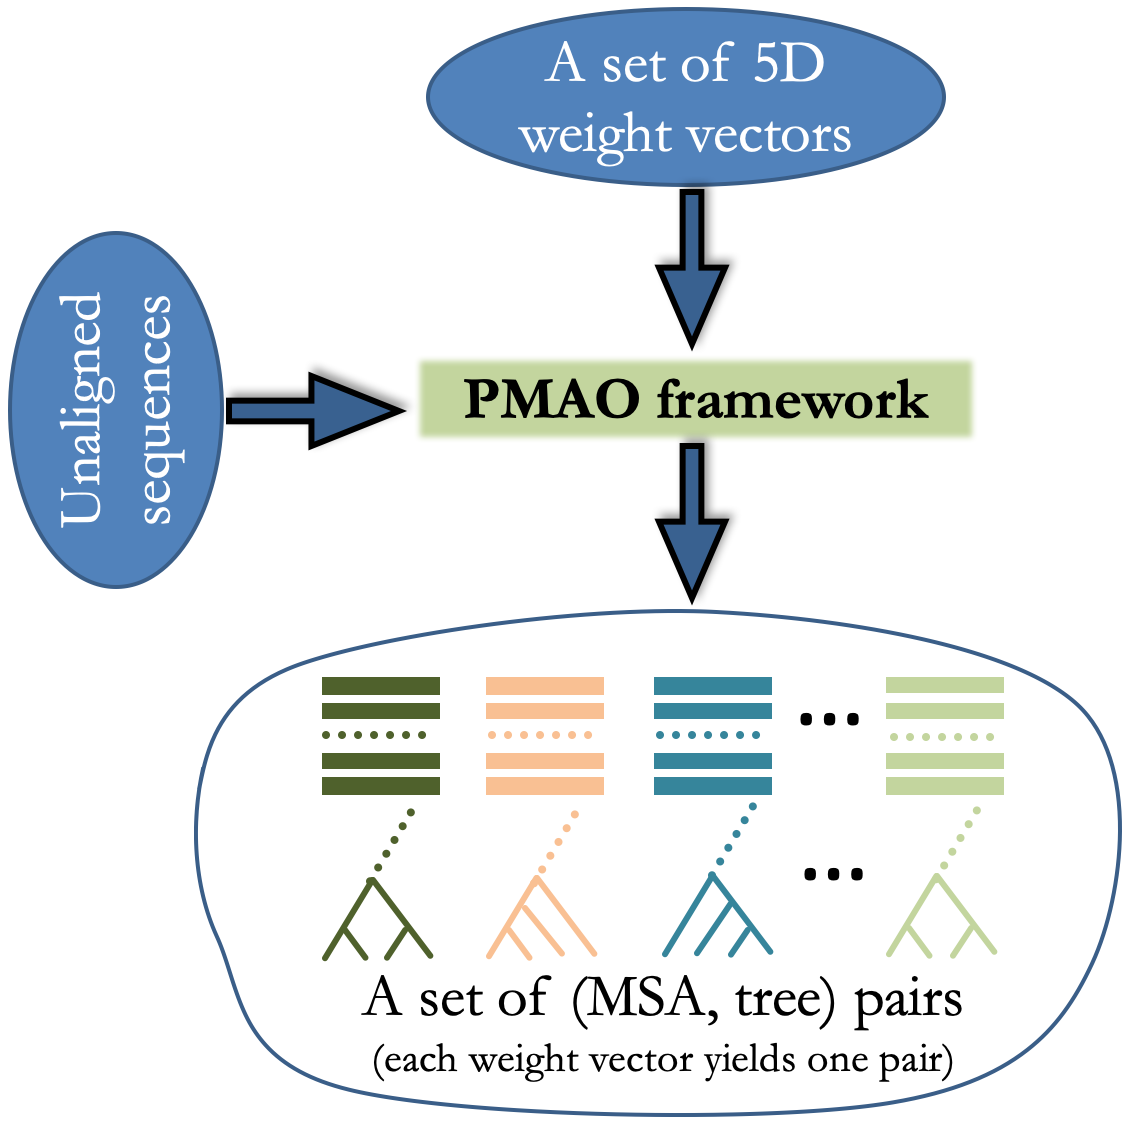
\includegraphics[width=\textwidth]{PMAO}
			\caption{Input-output}
	   \end{subfigure}		
%		\begin{subfigure}[b]{0.35\textwidth}
%			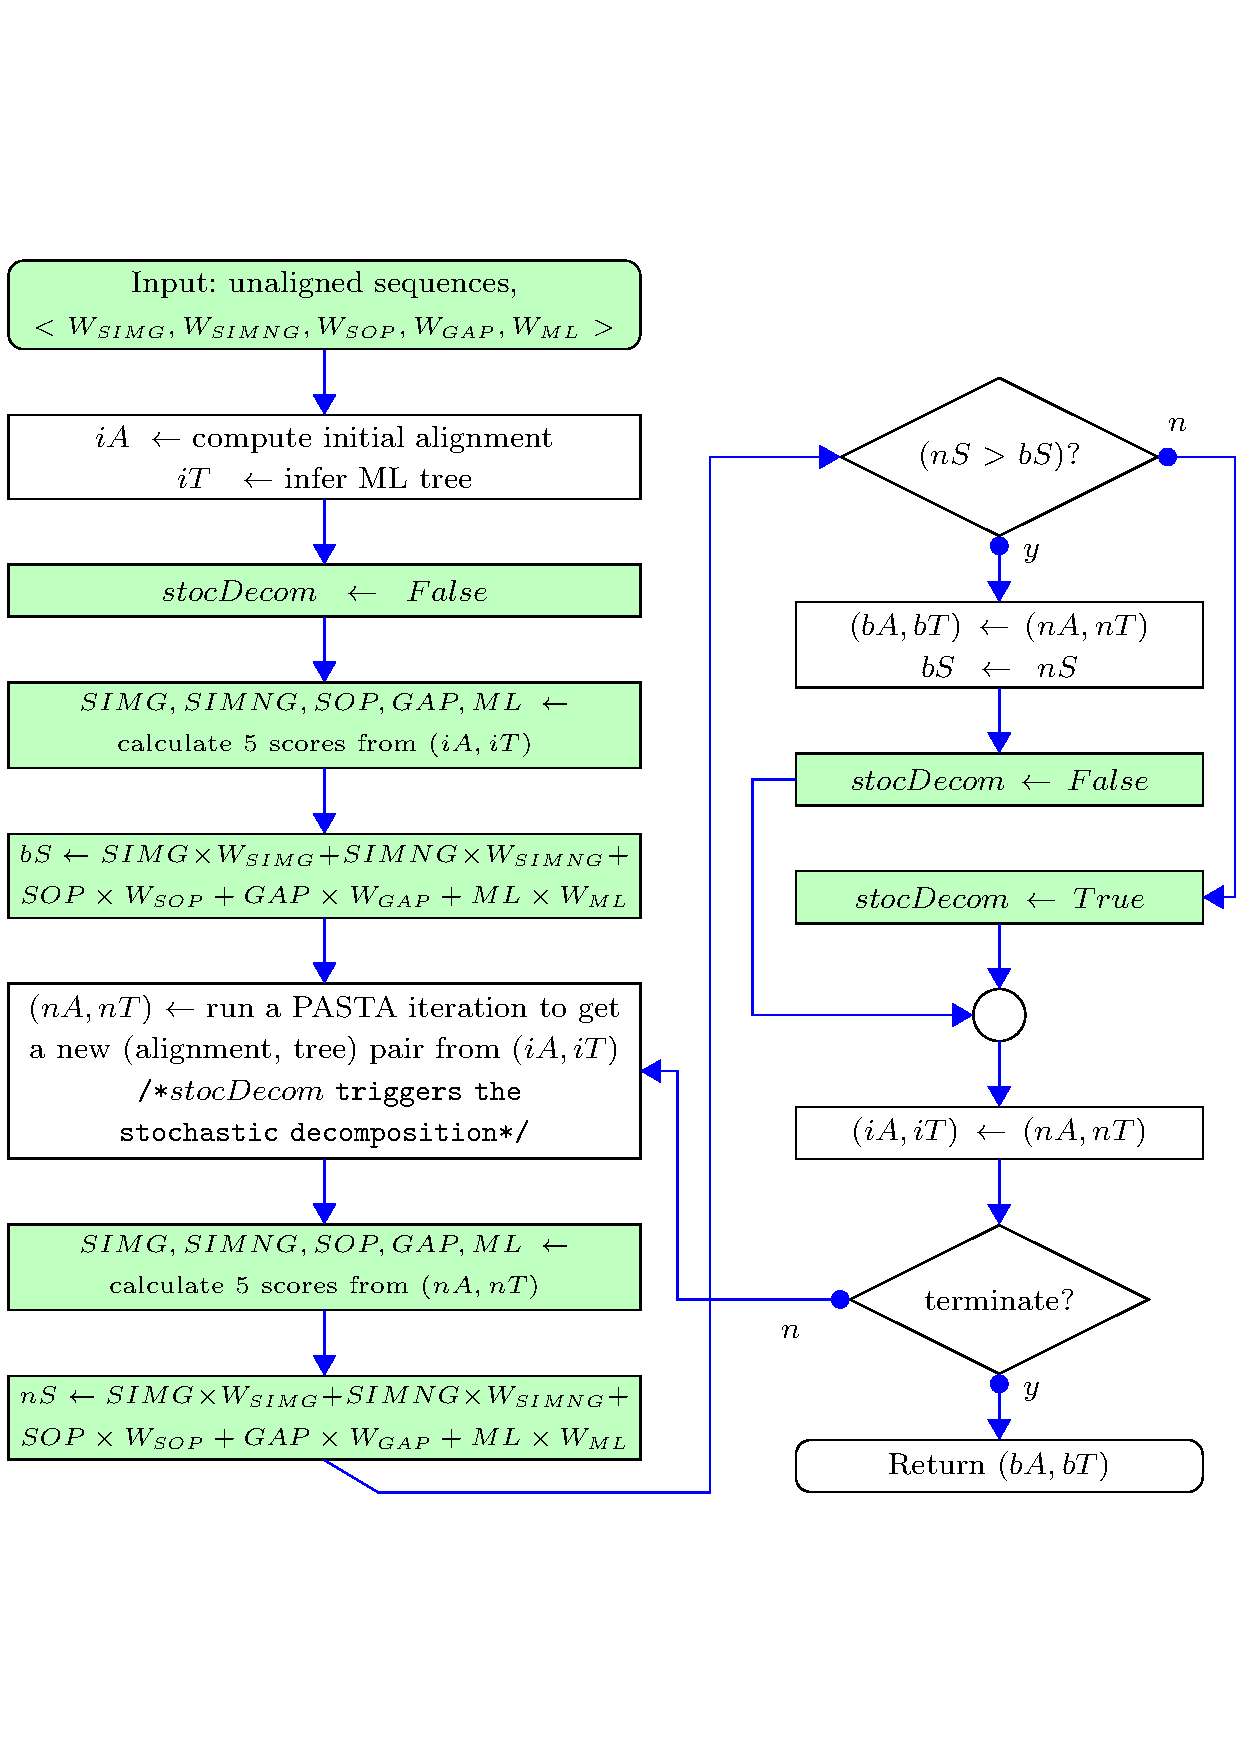
\includegraphics[width=\textwidth]{pmao-flow}
%			\caption{A high-level workflow for one weight vector}	
%			\label{fig:PMAO:flow}	
%		\end{subfigure}
		\begin{subfigure}[b]{0.5\textwidth}
		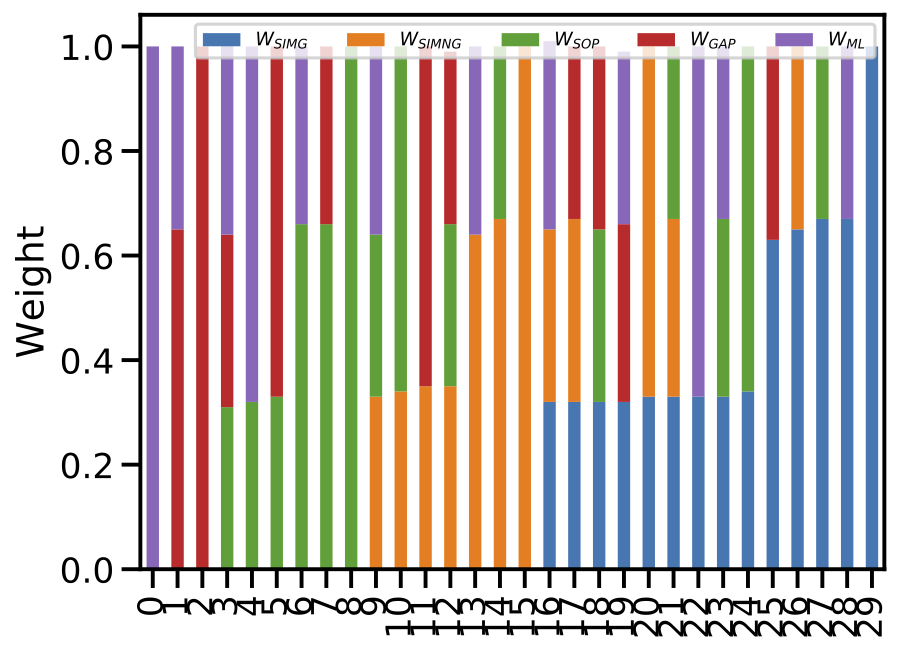
\includegraphics[width=\textwidth]{30-weight}
		\caption{30 well-spaced 5D weight vectors}
		\label{fig:weight}
		\end{subfigure}
	\end{adjustwidth}
	\caption{An overview of our PMAO framework.}
	\label{fig:PMAO}
\end{figure*}

\begin{figure}[!htbp]
	\centering
	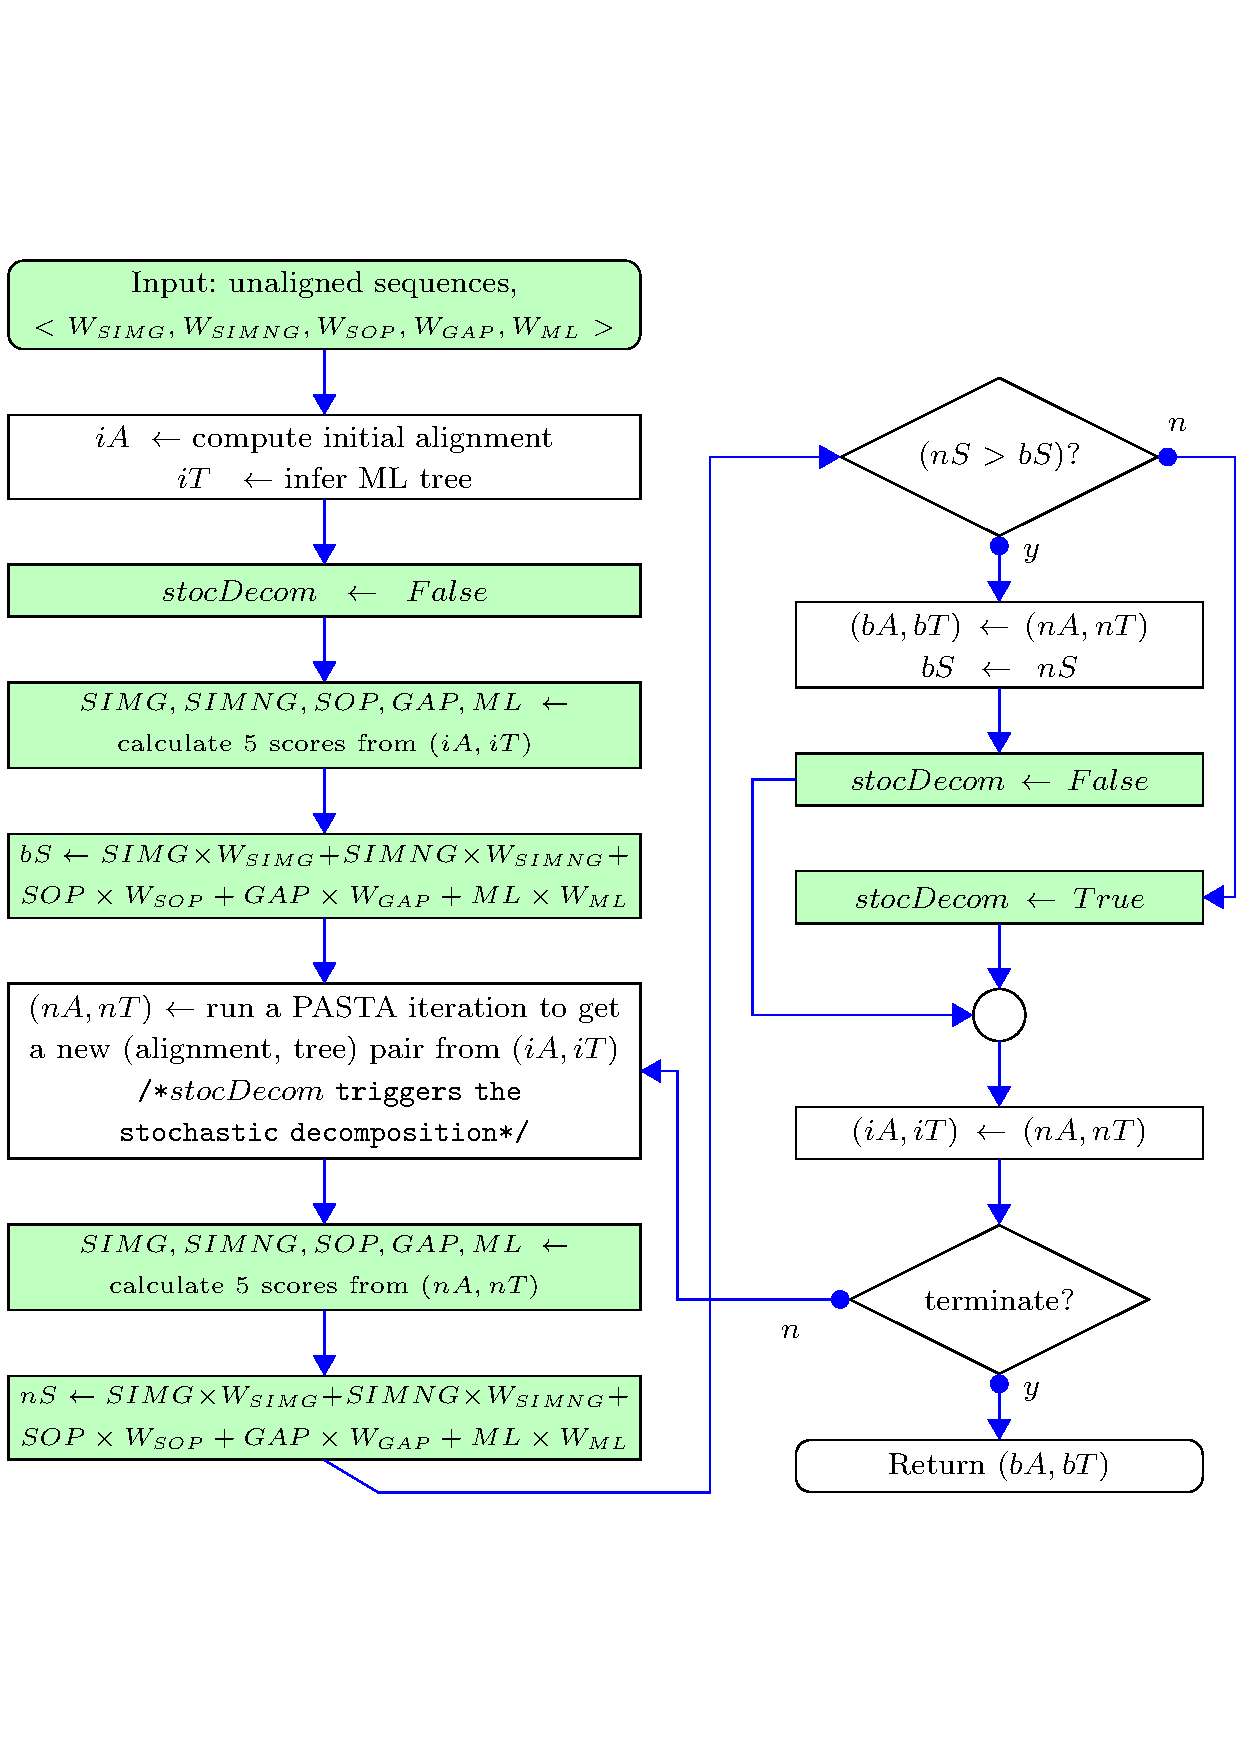
\includegraphics[width=0.9\textwidth]{pmao-flow}
	\caption{A high-level workflow of PMAO framework for one weight vector.}
	\label{fig:PMAO:flow}
\end{figure}

\subsection{Application-aware objective functions}
Alongside the ML score, we incorporate the following four simple objective functions, identified in Chapter~\ref{ch:cybernatics}based on their better correlation to the tree accuracy, in our PAMO framework. Several pairs of these objectives may have conflicting relationship as demonstrated in Chapter~\ref{ch:cybernatics}.
\begin{enumerate}
	\item Maximize similarity for columns containing gaps (SIMG): For each column of the MSA having at least one gap, it calculates the ratio of the most frequent characters. Then all those ratios are added to get the SIMG score.
	\item Maximize similarity for columns containing no gaps (SIMNG): This is similar to SIMG except that it considers those columns of the MSA that do not have any gap.
	\item Maximize sum-of-pairs (SOP): For each pair of aligned sequences in the MSA, it takes the sum of substitution score for the two aligned characters across all columns using a substitution matrix. The addition of all pairwise scores gives the SOP score. In this chapter, we use the BLOSUM62 matrix for protein sequences.
	\item Minimize the number of gaps (GAP): The summation of the number of gap characters in each aligned sequence. For the sake of uniformity, we convert this score into a maximization criterion.
\end{enumerate}


\subsection{PMAO framework}
\subsubsection{MO principles}
The goal of an MO algorithm is to generate a set of solutions, popularly known as the Pareto-optimal solutions in the MO literature, which represent the best compromise among the (conflicting) objectives.
Among the several classes of MO algorithms (e.g., pareto-based, decomposition-based, indicator-based, etc.), decomposition-based strategies are found effective to face the difficulties in handling `many' (i.e., more than three) objectives~\cite{li2015many}. These algorithms decompose the task of generating several alternative solutions into many single-objective problems with the help of a set of well-distributed weight vectors, popularly known as reference directions. Each weight vector aggregates the different objective scores into a single value that eventually leads to one member of the final solution set.

\subsubsection{Simplified workflow}
We develop a decomposition-based MO framework, namely, PASTA with many application-aware objectives (PMAO) (Figure~\ref{fig:PMAO}) by driving the search process of PASTA with a total of five objectives directed by a 5D weight vector. Figure~\ref{fig:PMAO:flow} depicts a high-level workflow for one weight vector, where the steps inspired by the MO approach are marked as green. This workflow is executed for all weight vectors to get alternative solutions and can be performed independently in parallel. As will be evident later, PMAO treats a solution better than the other based on the weighted-sum of five objective values instead of using ML score alone. Also, note that PMAO keeps track of whether an improved solution is generated at the previous iteration through a boolean variable \textit{stocDecom}. It impacts the divide-and-conquer strategy within PASTA by enabling the stochastic decomposition, which will be discussed soon. PMAO uses the default behavior of PASTA unless mentioned otherwise.

\subsubsection{Weight vectors}
Although working with a higher number of weight vectors increase the chance of getting better solutions in the solution set, we choose to work with 30 weight vectors to reduce the computational burden as well as to demonstrate the synergy between PASTA and an MO approach since 30 is quite a low number to tackle 5 objectives alone by an MO algorithm~\cite{deb2014evolutionary}. We calculate 30 well-spaced points on a 5D unit simplex using the method suggested by~\cite{ref_dirs_energy} as our weight vectors. Each of the 30 vertical bars in Figure~\ref{fig:weight} depicts one weight vector. 

\begin{algorithm}[!htbp]%\scriptsize
	\textbf{Input:} $tree$: to be bisected; $maxSize$: max. allowable leaves in a tree; $stocDecom$: triggers the stochastic decomposition
\begin{algorithmic}[1]
		\caption{min-cluster-size-bisect}
		\label{algo:min-bisect}
		\State{$nodeLeaves \gets$  empty dictionary}
		\For{each node $b$ in post-order-traverse($tree$)}
		\For{each child $c$ of node $b$}
		\State $nodeLeaves[ch] \gets $ \Call{leaf-count}{$ch$}
		\EndFor
		\If{ \Call{leaf-count}{$b$} $> maxSize$}
		\If{$stocDecom = False$}
		\State $selected \gets$ the node $x$ with the maximum $nodeLeaves[x]$ value
		\Else
		\State $selected \gets $ fitness proportionate selection where selection probability of a node $x \propto nodeLeaves[x]$ \Comment{stocastic decompostion} \label{algo:min-bisect:stoc}
		\EndIf
		\EndIf
		\State $t1 \gets $ the subtree of $tree$ rooted at $selected$
		\State remove $selected$ from its parent in $tree$
		\EndFor
		\State \textbf{return} $tree, t1$
		\Statex

		\Function{leaf-count}{$node$, $tree$}
		\State $ count $ $\gets$ no. of leaves in the subtree of $tree$ rooted at $node$
		\State \textbf{return} $ count $
		\EndFunction
	\end{algorithmic}
\end{algorithm}

\subsubsection{Stochastic decomposition}\label{subsec:stocastic}
We also enhance PASTA's divide-and-conquer method in the context of MO principles due to its huge impact on the accuracy of the generated (MSA, tree) pair~\cite{liu2012sate}. The heart of this strategy is a decomposition method that divides the leaves (i.e., unaligned sequences) of the guide tree into disjoint subsets. Since version 1.8.0, PASTA has been using \textit{mincluster} decomposition~\cite{balaban2019treecluster} which minimizes the number of resultant subsets given the maximum allowable members in a subset (\textit{maxSize} parameter in Algorithm~\ref{algo:min-bisect}). The default value of this parameter is set to half of the total leaf count. \textit{mincluster} strategy is implemented by repeatedly calling a method, namely, \textit{min-cluster-size-bisect}, to bisect a given tree. Scanning the nodes of the input tree in a post-order manner, it removes the subtree with the maximum number of leaves not exceeding the \textit{maxSize}. We embed some randomness in this method to (i) help PASTA to escape local optima and to (ii) increase the diversity of the solution set generated by PMAO. Line~\ref{algo:min-bisect:stoc} of Algorithm~\ref{algo:min-bisect} enforce the idea of stochastic decomposition, which randomly picks a subtree with the selection probability proportional to the number of leaves under that subtree.

\begin{algorithm}[!htbp]%\scriptsize
	\textbf{Input:} $SIMG, SIMNG, SOP, GAP, ML$: scores to be normalized
\begin{algorithmic}[1]
		\caption{rough-normalization}
		\label{algo:normalize}
		\State $GAP \gets 1.0/GAP$ \Comment{convert into a maximiation score}
		\State $ML \gets -1.0/ML$ \Comment{shift the value range to positive zone}
		\State $ obj \gets [SIMG, SIMNG, SOP, GAP, ML]$
		\State $max \gets$ the maximum value in $obj$
		\State $max \gets$ cast $max$ as integer
		\State $d \gets$ the no. of digits in $max$
		\State $ base \gets 10^{d+1}$
		\State add $base$ to all values in $obj$
		\For{$i \gets$ 0 to 4}
		\State $obj[i] \gets $ \Call{softsign}{$obj[i]$}
		\EndFor
		\State \textbf{return} $obj$
		\Statex

		\Function{softsign}{$x$} \label{algo:normalize:softsign}
		\State \textbf{return} $ \frac{x}{1 + |x|} $
		\EndFunction
	\end{algorithmic}
\end{algorithm}

\begin{figure}[!htbp]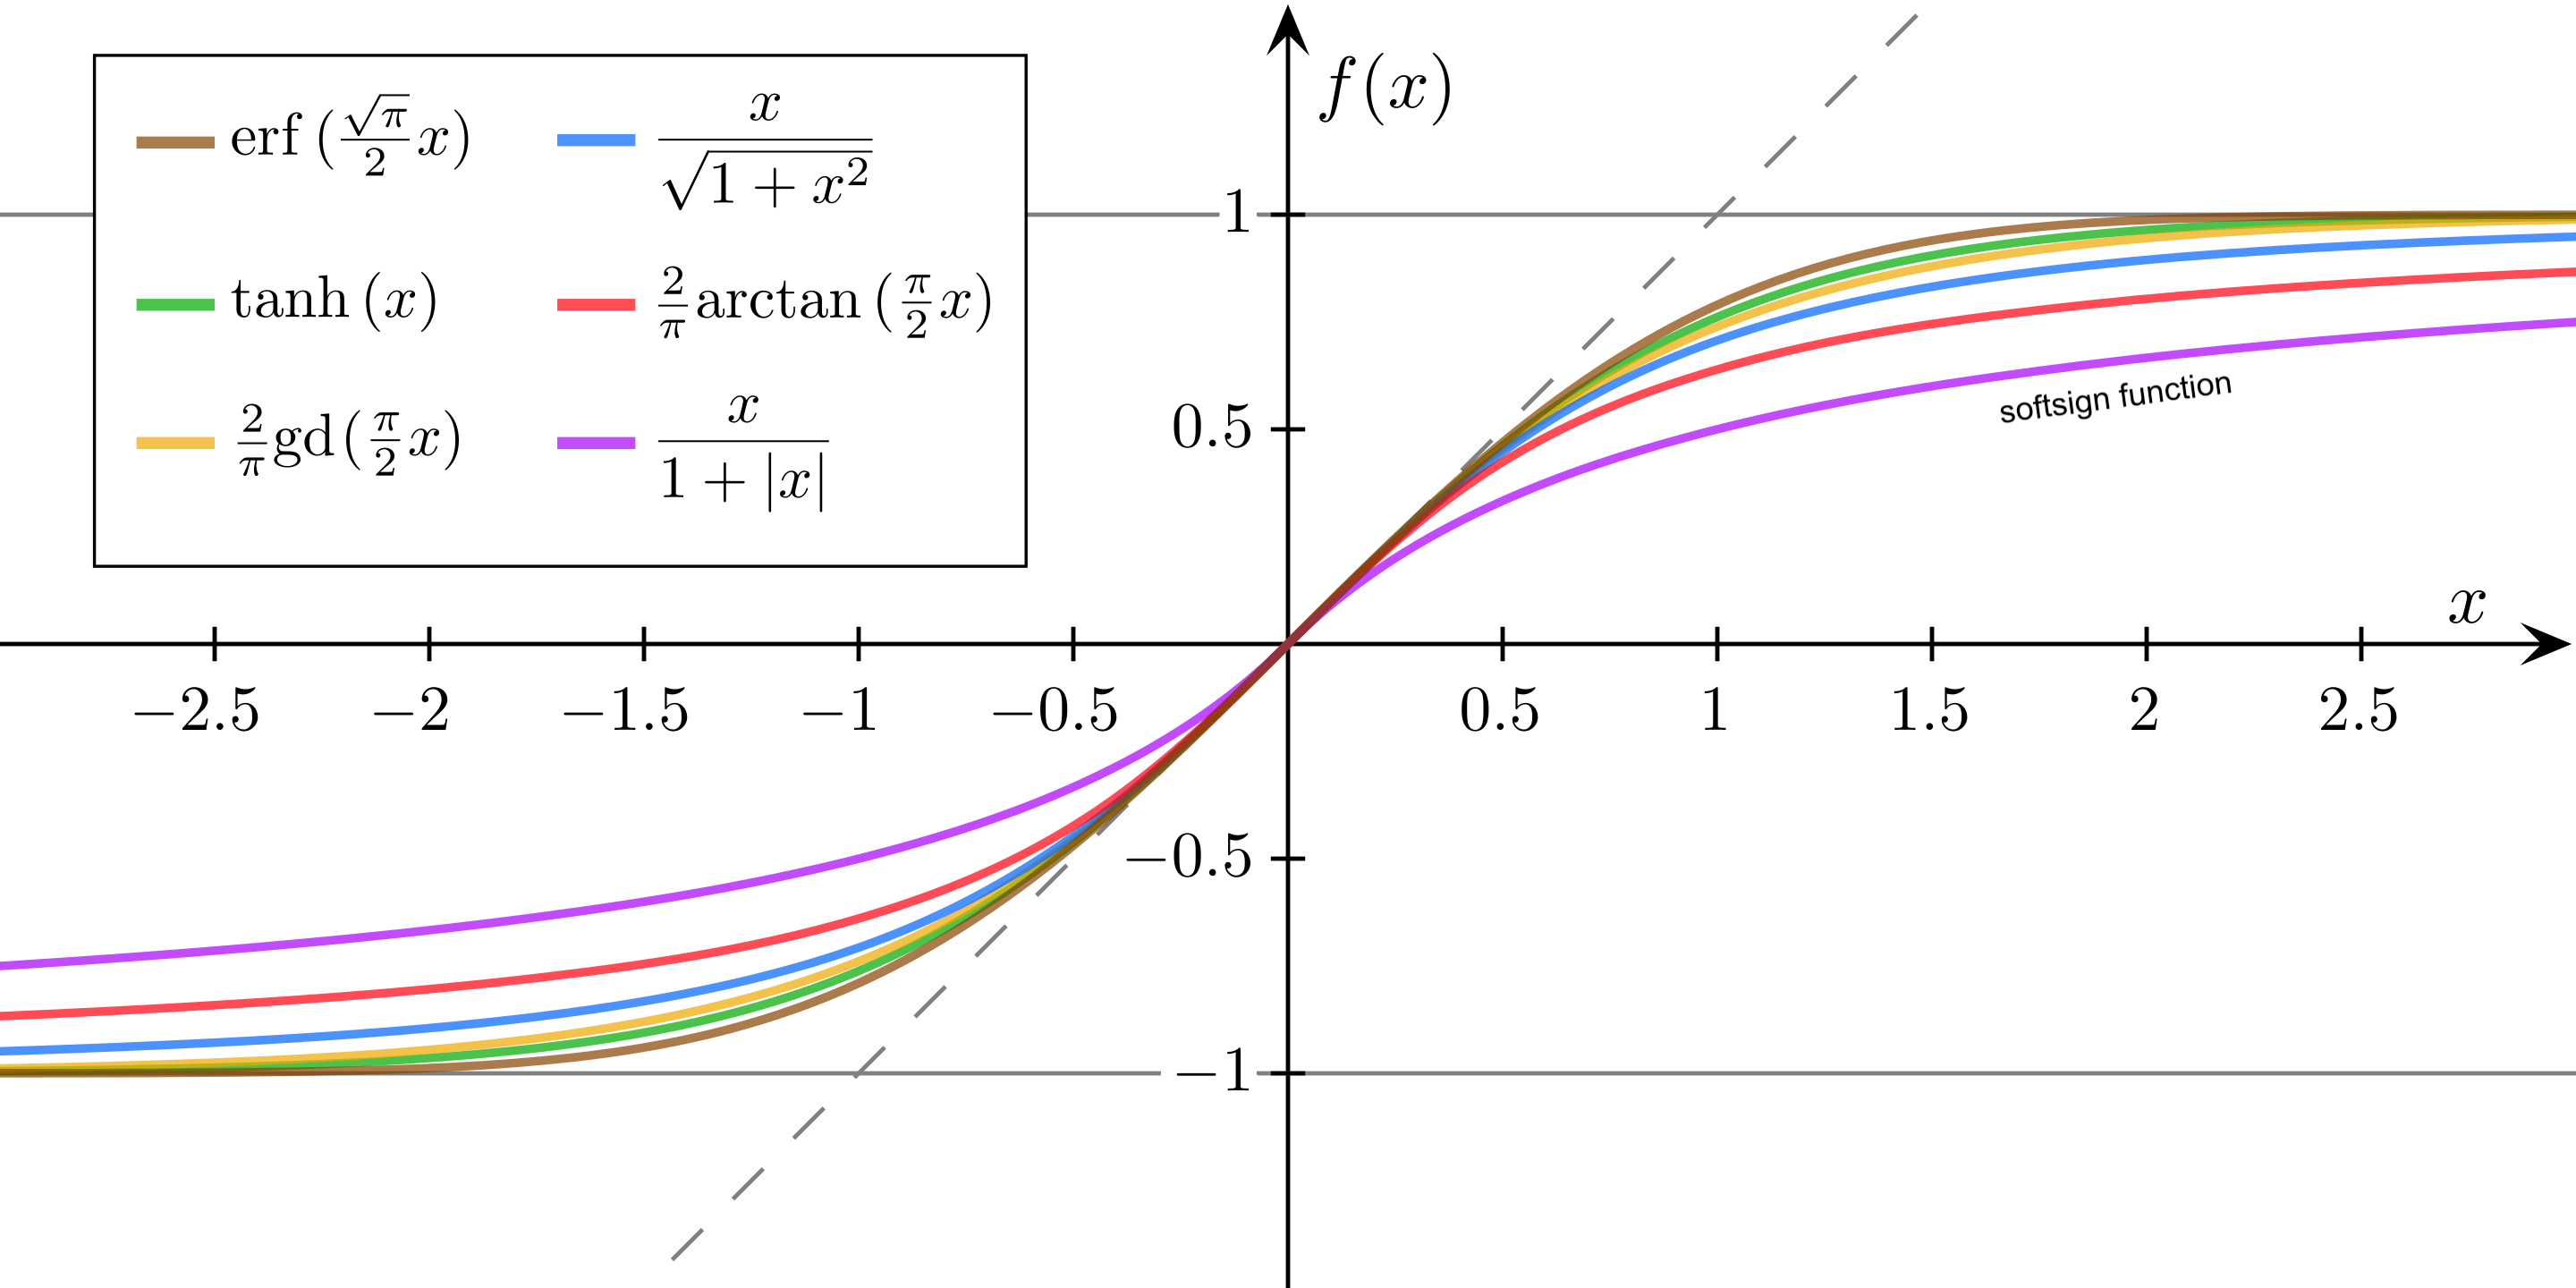
\includegraphics[width=0.8\textwidth]{sigmoid}
	\centering
	\caption{Some sigmoid functions. Image borrowed from WIKIPEDIA.}
	\label{fig:sigmoid}
\end{figure}

\subsubsection{Normalization}
Each of the five objective functions is measured using different scales, and their ranges differ to a great extent. So without normalization, their weighted-sum may be unexpectedly biased towards the objectives whose range extends far right, on the real number line, to the others. To add further complication, we do not have enough information regarding those objective values' distribution (e.g., min, max, avg, etc.). So we design a \textit{rough-normalization} method outlined in Algorithm~\ref{algo:normalize} which is called before the aggregation. Here we first transform the objective values to have the equal number of integer digits by adding an offset. Then we apply the softsign function (line~\ref{algo:normalize:softsign}) on each transformed value to make them close to 1.0. We choose the softsign function, over other sigmoid functions (Figure~\ref{fig:sigmoid}), as it converges polynomially (rather than exponentially) which helps to reduce further the risk of the aggregation being unjustly biased towards some objectives. 


\subsection{Domain-specific performance measure}
As we consider phylogeny estimation as the application domain of MSA, we assess the performance of PMAO solely based on the ML trees from its solution set. Therefore, we evaluate the quality of each ML tree with respect to the true phylogenetic tree
using a widely used measure known as the False Negative (FN) rate. FN rate is the percentage of edges present in the true tree but missing in the estimated tree. So a smaller value of the FN rate is desirable. Although there are two more common tree error measures: False Positive rate and Robinson-Foulds rate, all of them are identical when the true and estimated trees are binary~\cite{warnow2017computational} trees, which is the case in this thesis.


\subsection{Datasets}
We conduct our experiments on the BAliBASE 3.0 benchmark~\cite{thompson2005balibase} which is the most widely used alignment database of protein families. It provides manually refined reference alignments of high quality based on 3D structural superposition. For the sake of ease, we repeat that, BAliBASE 3.0 has 218 datasets which are organized into six groups according to their families and similarities: RV11 (very divergent sequences, residue identity below 20\%), RV12 (medium to divergent sequences, 20\%-40\% residue identity), RV20 (families with one or more highly divergent sequences), RV30 (divergent subfamilies), RV40 (sequences with large terminal N/C extensions), and RV50 (sequences with large internal insertions). To compare among different variants of PASTA and PMAO, we randomly sample 51 datasets in a stratified way within six groups. We divide them into set A and set B (listed by Table~\ref{tab:pmao-balibase}) for ease of presentation. Notably, in this chapter we primarily focused on improving the accuracy of PASTA and hence designed our experiments accordingly. We did not experiment scalability by working on larger datasets as PASTA is considered as a highly scalable tool.

\begin{table}[!htbp]
	\centering
	\small
	\caption{ Datasets selected randomly from BAliBASE 3.0 benchmark.}
	%\begin{adjustwidth}{-0.5cm}{}
	\begin{tabular}{|l|L{6.5cm}|L{6.5cm}|}
		\hline
		\multicolumn{1}{|c|}{Group} & Set A & Set B \\
		\hline
		RV11  & BB11005, BB11018, BB11020, BB11033 & BB11007, BB11019, BB11034, BB11038 \\
		\hline
		RV12  & BB12001, BB12013, BB12022, BB12035, BB12044 & BB12005, BB12026, BB12029,  BB12037\\
		\hline
		RV20  & BB20001, BB20010, BB20022, BB20033, BB20041 & BB20002, BB20012, BB20030, BB20037\\
		\hline
		RV30  & BB30002, BB30008, BB30015, BB30022 & BB30003 BB30011, BB30021, BB30026\\
		\hline
		RV40  & BB40001, BB40013, BB40025, BB40038, BB40048 & BB40006, BB40009, BB40019, BB40033 \\ \hline
		RV50  & BB50001, BB50005, BB50010, BB50016 &  BB50006 BB50002, BB50009, BB50014 \\
		\hline
	\end{tabular}\label{tab:pmao-balibase}
	%\end{adjustwidth}
\end{table}

As we adopt the FN rate as our domain-specific performance measure, following the strategy of~\cite{mirarab2015pasta} we generate a reference tree for each dataset by inferring an ML tree from the reference alignments using RAxML~\cite{stamatakis2014raxml} with bootstrapping and retaining only the highly supported edges.

 \section{Results and discussion}
\label{sec:experiment}

\subsection{Impact of stochastic decomposition}
To assess the impact of the underlying stochastic decomposition method on PMAO, we create four variants of PMAO and PASTA (Table~\ref{tab:pmao-variants}). In particular, we vary the number of iterations and consider both \textit{mincluster} based (i.e., the default for PASTA) and stochastic decomposition. Increasing the iteration potentially intensifies the effect of the stochastic decomposition in PMAO framework. In Tables~\ref{tab:pmao-variants-a},  \ref{tab:pmao-variants-b}, we report the best FN rates among the 30 solutions generated by PMAO variants for datasets under set A and B, respectively; lower (i.e., better) FN rate values are marked with a darker shade.
We observe that the PMAO-3I-S and PMAO-8I-S columns contain more darker shades than PMAO-3I-D and PMAO-8I-D columns, which indicates the positive impact of stochastic decomposition on the performance of PMAO framework. To contrast among these variants, we apply the Friedman Aligned Ranks test~\cite{hodges2012rank} followed by complementary Holm’s post-hoc procedure~\cite{holm1979simple} on Tables~\ref{tab:pmao-variants-a},  \ref{tab:pmao-variants-b}, as recommended by~\cite{derrac2011practical, rodriguez-fdez2015stac} using 95\% confidence level. The results the summarized in Table~\ref{tab:test-pmao-variants}. The lower ranks of stochastic variants and significant difference between PMAO-3I-D and PMAO-8I-S suggest the effectiveness of stochastic decomposition. Note that PASTA uses three iterations by default, and most of its improvement is achieved in the first iteration. So, increasing iteration is not expected to improve PASTA output significantly. Moreover, stochastic decomposition makes sense in the context of MO principles as discussed earlier in Section~\ref{subsec:stocastic}. We have verified this by conducting similar analyses (Supplementary Tables~\ref{tab:pasta-variants-a}, \ref{tab:pasta-variants-b},  \ref{tab:test-pasta-variants} in Appendix~\ref{apendix:pmao}) based on four PASTA variants. The PASTA-3I-S variant does not get ample opportunity to leverage the stochastic decomposition due to its single execution.
In contrast, the PMAO-3I-S variant executes that 30 times on different search spaces defined by the weight vectors. We find no significant difference between any pair of PASTA variants as expected (Supplementary Table~\ref{tab:test-pasta-variants} in Appendix~\ref{apendix:pmao}), and PASTA-8I-D seems to be the best variant (more darker shades). In the subsequent sections, we use the PMAO-8I-S and the PASTA-8I-D variants for a fair comparison.


\begin{table}[!htbp]
  \centering
  \caption{PMAO and PASTA variants based on iteration count and guide tree decomposition strategy.}
    \begin{tabular}{c|l|r|l}
    \multicolumn{1}{l|}{Method} & Variant & \multicolumn{1}{l|}{Iteration} & Tree decomposition\\
    \hline
    \multirow{4}{*}{PMAO} & PMAO-3I-D  & 3     & Default (\textit{mincluster}) \\
	\cline{2-4}          & 	PMAO-8I-D  & 8     & Default (\textit{mincluster}) \\
	\cline{2-4}          & PMAO-3I-S  & 3     & Stochastic \\
	\cline{2-4}          & PMAO-8I-S  & 8     & Stochastic\\
	\hline \hline
	    \multirow{4}{*}{PASTA} & PMAO-3I-D  & 3     & Default (\textit{mincluster}) \\
	\cline{2-4}          & PASTA-8I-D  & 8     & Default (\textit{mincluster}) \\
	\cline{2-4}          & PASTA-3I-S  & 3     & Stochastic \\
	\cline{2-4}          & PASTA-8I-S  & 8     & Stochastic\\
    \hline
    \end{tabular}\label{tab:pmao-variants}\end{table}


\begin{table}[!htbp]
\begin{adjustwidth}{-0.6cm}{}
	\centering
	\scriptsize
	\caption{Best FN rate achieved by the four variants of PMAO for each dataset in set A. On each row, the lower (better) FN rates are marked with darker shade.}
	\begin{tabular}{|l|r|r|r|r|}
		\hline
		\multirow{2}{*}{Dataset} & \multicolumn{4}{c|}{Best FN rates achieved by PMAO variants} \\
		\cline{2-5}          & PMAO-3I-D & PMAO-8I-D & PMAO-3I-S & PMAO-8I-S \\
		\hline
		BB11005 & \cellcolor[rgb]{ .988,  1,  .992}0.18 & \cellcolor[rgb]{ .384,  .745,  .478}0.09 & \cellcolor[rgb]{ .384,  .745,  .478}0.09 & \cellcolor[rgb]{ .384,  .745,  .478}0.09 \\
		\hline
		BB11018 & \cellcolor[rgb]{ .988,  1,  .992}0.27 & \cellcolor[rgb]{ .384,  .745,  .478}0.18 & \cellcolor[rgb]{ .384,  .745,  .478}0.18 & \cellcolor[rgb]{ .384,  .745,  .478}0.18 \\
		\hline
		BB11033 & \cellcolor[rgb]{ .988,  1,  .992}0.38 & \cellcolor[rgb]{ .988,  1,  .992}0.38 & \cellcolor[rgb]{ .988,  1,  .992}0.38 & \cellcolor[rgb]{ .988,  1,  .992}0.38 \\
		\hline
		BB11020 & \cellcolor[rgb]{ .988,  1,  .992}0.33 & \cellcolor[rgb]{ .988,  1,  .992}0.33 & \cellcolor[rgb]{ .988,  1,  .992}0.33 & \cellcolor[rgb]{ .988,  1,  .992}0.33 \\
		\hline
		BB12001 & \cellcolor[rgb]{ .988,  1,  .992}0.13 & \cellcolor[rgb]{ .988,  1,  .992}0.13 & \cellcolor[rgb]{ .988,  1,  .992}0.13 & \cellcolor[rgb]{ .988,  1,  .992}0.13 \\
		\hline
		BB12013 & \cellcolor[rgb]{ .384,  .745,  .478}0.00 & \cellcolor[rgb]{ .988,  1,  .992}0.20 & \cellcolor[rgb]{ .384,  .745,  .478}0.00 & \cellcolor[rgb]{ .988,  1,  .992}0.20 \\
		\hline
		BB12022 & \cellcolor[rgb]{ .988,  1,  .992}0.00 & \cellcolor[rgb]{ .988,  1,  .992}0.00 & \cellcolor[rgb]{ .988,  1,  .992}0.00 & \cellcolor[rgb]{ .988,  1,  .992}0.00 \\
		\hline
		BB12035 & \cellcolor[rgb]{ .988,  1,  .992}0.04 & \cellcolor[rgb]{ .384,  .745,  .478}0.00 & \cellcolor[rgb]{ .988,  1,  .992}0.04 & \cellcolor[rgb]{ .988,  1,  .992}0.04 \\
		\hline
		BB12044 & \cellcolor[rgb]{ .988,  1,  .992}0.38 & \cellcolor[rgb]{ .988,  1,  .992}0.38 & \cellcolor[rgb]{ .988,  1,  .992}0.38 & \cellcolor[rgb]{ .988,  1,  .992}0.38 \\
		\hline
		BB20001 & \cellcolor[rgb]{ .384,  .745,  .478}0.23 & \cellcolor[rgb]{ .988,  1,  .992}0.46 & \cellcolor[rgb]{ .384,  .745,  .478}0.23 & \cellcolor[rgb]{ .384,  .745,  .478}0.23 \\
		\hline
		BB20010 & \cellcolor[rgb]{ .988,  1,  .992}0.31 & \cellcolor[rgb]{ .988,  1,  .992}0.31 & \cellcolor[rgb]{ .384,  .745,  .478}0.08 & \cellcolor[rgb]{ .384,  .745,  .478}0.08 \\
		\hline
		BB20022 & \cellcolor[rgb]{ .988,  1,  .992}0.11 & \cellcolor[rgb]{ .988,  1,  .992}0.11 & \cellcolor[rgb]{ .988,  1,  .992}0.11 & \cellcolor[rgb]{ .384,  .745,  .478}0.09 \\
		\hline
		BB20033 & \cellcolor[rgb]{ .988,  1,  .992}0.36 & \cellcolor[rgb]{ .988,  1,  .992}0.36 & \cellcolor[rgb]{ .988,  1,  .992}0.36 & \cellcolor[rgb]{ .384,  .745,  .478}0.24 \\
		\hline
		BB20041 & \cellcolor[rgb]{ .988,  1,  .992}0.33 & \cellcolor[rgb]{ .584,  .827,  .647}0.29 & \cellcolor[rgb]{ .384,  .745,  .478}0.27 & \cellcolor[rgb]{ .988,  1,  .992}0.33 \\
		\hline
		BB30002 & \cellcolor[rgb]{ .988,  1,  .992}0.32 & \cellcolor[rgb]{ .988,  1,  .992}0.32 & \cellcolor[rgb]{ .384,  .745,  .478}0.14 & \cellcolor[rgb]{ .502,  .792,  .58}0.18 \\
		\hline
		BB30008 & \cellcolor[rgb]{ .533,  .808,  .604}0.24 & \cellcolor[rgb]{ .988,  1,  .992}0.33 & \cellcolor[rgb]{ .835,  .933,  .863}0.30 & \cellcolor[rgb]{ .384,  .745,  .478}0.21 \\
		\hline
		BB30015 & \cellcolor[rgb]{ .988,  1,  .992}0.17 & \cellcolor[rgb]{ .988,  1,  .992}0.17 & \cellcolor[rgb]{ .988,  1,  .992}0.17 & \cellcolor[rgb]{ .988,  1,  .992}0.17 \\
		\hline
		BB30022 & \cellcolor[rgb]{ .682,  .871,  .733}0.48 & \cellcolor[rgb]{ .682,  .871,  .733}0.48 & \cellcolor[rgb]{ .988,  1,  .992}0.49 & \cellcolor[rgb]{ .384,  .745,  .478}0.46 \\
		\hline
		BB40001 & \cellcolor[rgb]{ .988,  1,  .992}0.48 & \cellcolor[rgb]{ .784,  .914,  .82}0.44 & \cellcolor[rgb]{ .988,  1,  .992}0.48 & \cellcolor[rgb]{ .384,  .745,  .478}0.36 \\
		\hline
		BB40013 & \cellcolor[rgb]{ .988,  1,  .992}0.31 & \cellcolor[rgb]{ .988,  1,  .992}0.31 & \cellcolor[rgb]{ .988,  1,  .992}0.31 & \cellcolor[rgb]{ .384,  .745,  .478}0.25 \\
		\hline
		BB40025 & \cellcolor[rgb]{ .988,  1,  .992}0.00 & \cellcolor[rgb]{ .988,  1,  .992}0.00 & \cellcolor[rgb]{ .988,  1,  .992}0.00 & \cellcolor[rgb]{ .988,  1,  .992}0.00 \\
		\hline
		BB40038 & \cellcolor[rgb]{ .988,  1,  .992}0.10 & \cellcolor[rgb]{ .988,  1,  .992}0.10 & \cellcolor[rgb]{ .988,  1,  .992}0.10 & \cellcolor[rgb]{ .988,  1,  .992}0.10 \\
		\hline
		BB40048 & \cellcolor[rgb]{ .988,  1,  .992}0.29 & \cellcolor[rgb]{ .988,  1,  .992}0.29 & \cellcolor[rgb]{ .384,  .745,  .478}0.21 & \cellcolor[rgb]{ .988,  1,  .992}0.29 \\
		\hline
		BB50001 & \cellcolor[rgb]{ .988,  1,  .992}0.29 & \cellcolor[rgb]{ .988,  1,  .992}0.29 & \cellcolor[rgb]{ .988,  1,  .992}0.29 & \cellcolor[rgb]{ .988,  1,  .992}0.29 \\
		\hline
		BB50005 & \cellcolor[rgb]{ .686,  .871,  .733}0.25 & \cellcolor[rgb]{ .988,  1,  .992}0.38 & \cellcolor[rgb]{ .384,  .745,  .478}0.13 & \cellcolor[rgb]{ .686,  .871,  .733}0.25 \\
		\hline
		BB50010 & \cellcolor[rgb]{ .988,  1,  .992}0.07 & \cellcolor[rgb]{ .384,  .745,  .478}0.00 & \cellcolor[rgb]{ .384,  .745,  .478}0.00 & \cellcolor[rgb]{ .384,  .745,  .478}0.00 \\
		\hline
		BB50016 & \cellcolor[rgb]{ .682,  .871,  .733}0.13 & \cellcolor[rgb]{ .988,  1,  .992}0.20 & \cellcolor[rgb]{ .384,  .745,  .478}0.07 & \cellcolor[rgb]{ .384,  .745,  .478}0.07 \\
		\hline
	\end{tabular}\label{tab:pmao-variants-a}\end{adjustwidth}
\end{table}

\begin{table}[!htbp]
\centering
\scriptsize
\caption{Best FN rate achieved by the four variants of PMAO for each dataset in set B. On each row, the lower (better) FN rates are marked with darker shade.}
	\begin{tabular}{|l|r|r|r|r|}
		\hline
		\multirow{2}{*}{Dataset} & \multicolumn{4}{c|}{Best FN rates achieved by PMAO variants} \\
		\cline{2-5}          & \multicolumn{1}{l|}{PMAO-3I-D} & \multicolumn{1}{l|}{PMAO-8I-D} & \multicolumn{1}{l|}{PMAO-3I-S} & \multicolumn{1}{l|}{PMAO-8I-S} \\
		\hline
		BB11007 & \cellcolor[rgb]{ .384,  .745,  .478}0.33 & \cellcolor[rgb]{ .384,  .745,  .478}0.33 & \cellcolor[rgb]{ .988,  1,  .992}0.50 & \cellcolor[rgb]{ .384,  .745,  .478}0.33 \\
		\hline
		BB11034 & \cellcolor[rgb]{ .988,  1,  .992}0.20 & \cellcolor[rgb]{ .384,  .745,  .478}0.00 & \cellcolor[rgb]{ .988,  1,  .992}0.20 & \cellcolor[rgb]{ .988,  1,  .992}0.20 \\
		\hline
		BB11038 & \cellcolor[rgb]{ .384,  .745,  .478}0.00 & \cellcolor[rgb]{ .384,  .745,  .478}0.00 & \cellcolor[rgb]{ .988,  1,  .992}0.40 & \cellcolor[rgb]{ .384,  .745,  .478}0.00 \\
		\hline
		BB11019 & \cellcolor[rgb]{ .988,  1,  .992}0.14 & \cellcolor[rgb]{ .988,  1,  .992}0.14 & \cellcolor[rgb]{ .988,  1,  .992}0.14 & \cellcolor[rgb]{ .988,  1,  .992}0.14 \\
		\hline
		BB12005 & \cellcolor[rgb]{ .988,  1,  .992}0.33 & \cellcolor[rgb]{ .988,  1,  .992}0.33 & \cellcolor[rgb]{ .988,  1,  .992}0.33 & \cellcolor[rgb]{ .988,  1,  .992}0.33 \\
		\hline
		BB12029 & \cellcolor[rgb]{ .988,  1,  .992}0.44 & \cellcolor[rgb]{ .988,  1,  .992}0.44 & \cellcolor[rgb]{ .384,  .745,  .478}0.33 & \cellcolor[rgb]{ .384,  .745,  .478}0.33 \\
		\hline
		BB12026 & \cellcolor[rgb]{ .384,  .745,  .478}0.27 & \cellcolor[rgb]{ .384,  .745,  .478}0.27 & \cellcolor[rgb]{ .384,  .745,  .478}0.27 & \cellcolor[rgb]{ .988,  1,  .992}0.33 \\
		\hline
		BB12037 & \cellcolor[rgb]{ .988,  1,  .992}0.10 & \cellcolor[rgb]{ .988,  1,  .992}0.10 & \cellcolor[rgb]{ .988,  1,  .992}0.10 & \cellcolor[rgb]{ .988,  1,  .992}0.10 \\
		\hline
		BB20002 & \cellcolor[rgb]{ .686,  .871,  .733}0.53 & \cellcolor[rgb]{ .384,  .745,  .478}0.47 & \cellcolor[rgb]{ .988,  1,  .992}0.59 & \cellcolor[rgb]{ .686,  .871,  .733}0.53 \\
		\hline
		BB20012 & \cellcolor[rgb]{ .988,  1,  .992}0.29 & \cellcolor[rgb]{ .745,  .894,  .784}0.21 & \cellcolor[rgb]{ .745,  .894,  .784}0.21 & \cellcolor[rgb]{ .384,  .745,  .478}0.08 \\
		\hline
		BB20030 & \cellcolor[rgb]{ .988,  1,  .992}0.64 & \cellcolor[rgb]{ .384,  .745,  .478}0.50 & \cellcolor[rgb]{ .988,  1,  .992}0.64 & \cellcolor[rgb]{ .988,  1,  .992}0.64 \\
		\hline
		BB20037 & \cellcolor[rgb]{ .988,  1,  .992}0.13 & \cellcolor[rgb]{ .988,  1,  .992}0.13 & \cellcolor[rgb]{ .988,  1,  .992}0.13 & \cellcolor[rgb]{ .988,  1,  .992}0.13 \\
		\hline
		BB30003 & \cellcolor[rgb]{ .988,  1,  .992}0.27 & \cellcolor[rgb]{ .384,  .745,  .478}0.25 & \cellcolor[rgb]{ .682,  .871,  .733}0.26 & \cellcolor[rgb]{ .682,  .871,  .733}0.26 \\
		\hline
		BB30021 & \cellcolor[rgb]{ .729,  .89,  .769}0.30 & \cellcolor[rgb]{ .816,  .925,  .843}0.31 & \cellcolor[rgb]{ .384,  .745,  .478}0.27 & \cellcolor[rgb]{ .988,  1,  .992}0.32 \\
		\hline
		BB30026 & \cellcolor[rgb]{ .384,  .745,  .478}0.15 & \cellcolor[rgb]{ .384,  .745,  .478}0.15 & \cellcolor[rgb]{ .988,  1,  .992}0.17 & \cellcolor[rgb]{ .384,  .745,  .478}0.15 \\
		\hline
		BB30011 & \cellcolor[rgb]{ .988,  1,  .992}0.32 & \cellcolor[rgb]{ .384,  .745,  .478}0.31 & \cellcolor[rgb]{ .384,  .745,  .478}0.31 & \cellcolor[rgb]{ .384,  .745,  .478}0.31 \\
		\hline
		BB40009 & \cellcolor[rgb]{ .988,  1,  .992}0.13 & \cellcolor[rgb]{ .988,  1,  .992}0.13 & \cellcolor[rgb]{ .988,  1,  .992}0.13 & \cellcolor[rgb]{ .988,  1,  .992}0.13 \\
		\hline
		BB40019 & \cellcolor[rgb]{ .988,  1,  .992}0.29 & \cellcolor[rgb]{ .988,  1,  .992}0.29 & \cellcolor[rgb]{ .384,  .745,  .478}0.14 & \cellcolor[rgb]{ .988,  1,  .992}0.29 \\
		\hline
		BB40033 & \cellcolor[rgb]{ .988,  1,  .992}0.06 & \cellcolor[rgb]{ .988,  1,  .992}0.06 & \cellcolor[rgb]{ .988,  1,  .992}0.06 & \cellcolor[rgb]{ .988,  1,  .992}0.06 \\
		\hline
		BB40006 & \cellcolor[rgb]{ .988,  1,  .992}0.00 & \cellcolor[rgb]{ .988,  1,  .992}0.00 & \cellcolor[rgb]{ .988,  1,  .992}0.00 & \cellcolor[rgb]{ .988,  1,  .992}0.00 \\
		\hline
		BB50002 & \cellcolor[rgb]{ .384,  .745,  .478}0.40 & \cellcolor[rgb]{ .988,  1,  .992}0.50 & \cellcolor[rgb]{ .988,  1,  .992}0.50 & \cellcolor[rgb]{ .384,  .745,  .478}0.40 \\
		\hline
		BB50009 & \cellcolor[rgb]{ .988,  1,  .992}0.08 & \cellcolor[rgb]{ .988,  1,  .992}0.08 & \cellcolor[rgb]{ .988,  1,  .992}0.08 & \cellcolor[rgb]{ .988,  1,  .992}0.08 \\
		\hline
		BB50014 & \cellcolor[rgb]{ .988,  1,  .992}0.41 & \cellcolor[rgb]{ .988,  1,  .992}0.41 & \cellcolor[rgb]{ .988,  1,  .992}0.41 & \cellcolor[rgb]{ .384,  .745,  .478}0.26 \\
		\hline
		BB50006 & \cellcolor[rgb]{ .988,  1,  .992}0.16 & \cellcolor[rgb]{ .988,  1,  .992}0.16 & \cellcolor[rgb]{ .988,  1,  .992}0.16 & \cellcolor[rgb]{ .384,  .745,  .478}0.12 \\
		\hline
	\end{tabular}\label{tab:pmao-variants-b}\end{table}

\begin{table}[!htbp]
	\centering
	\small
	\caption[Friedman test and Holm's post-hoc procedure to assess the significance of difference among the PMAO variants.]{\underline{Friedman Aligned Ranks test (Column 2):} Friedman Aligned ranks (lower is better) of the four variants of PMAO based on Table~\ref{tab:pmao-variants-a},  \ref{tab:pmao-variants-b}. We also show the computed statistics and corresponding $ p $-value.
		\underline{Holm's post-hoc procedure (Columns 3 - 6):} Comparison among the PMAO variants using the Holm's post-hoc procedures. Each entry shows the adjusted $p$-value which indicates the significance of the difference in performance between two methods.}
	\begin{tabular}{|l|r||c|c|c|c|}
		\hline
		\multicolumn{1}{|c|}{1} & \multicolumn{1}{c||}{2} & \multicolumn{1}{c|}{3} & \multicolumn{1}{c|}{4} & \multicolumn{1}{c|}{5} & 6 \\
		\hline
		\multirow{2}{*}{\makecell{PMAO\\ variants}} & \multirow{2}{*}{\makecell{Friedman\\Aligned rank*}} & \multicolumn{4}{c|}{Holm's adjusted $p$-value} \\
		\cline{3-6}          &       & 8I-S & 3I-S & 8I-D & 3I-D \\
		\hline
		8I-S & 82.3137 & \multicolumn{1}{c|}{-} & \multicolumn{1}{r|}{0.4032} & \multicolumn{1}{r|}{0.1431} & \multicolumn{1}{r|}{\cellcolor[rgb]{ .384,  .745,  .478}0.0077} \\
		\hline
		3I-S & 99.8137 & \multicolumn{1}{r|}{0.4032} & \multicolumn{1}{c|}{-} & \multicolumn{1}{r|}{0.6038} & \multicolumn{1}{r|}{0.3387} \\
		\hline
		8I-D & 107.9020 & \multicolumn{1}{r|}{0.1431} & \multicolumn{1}{r|}{0.6038} & \multicolumn{1}{c|}{-} & \multicolumn{1}{r|}{0.6038} \\
		\hline
		3I-D & 119.9706 & \multicolumn{1}{r|}{\cellcolor[rgb]{ .384,  .745,  .478}0.0077} & \multicolumn{1}{r|}{0.3387} & \multicolumn{1}{r|}{0.6038} & - \\
		\hline
		*Statistic & 9.0393 & \multicolumn{4}{c|}{\multirow{2}{*}{N/A}} \\
		\cline{1-2}    *$p$-value & 0.0288 & \multicolumn{4}{c|}{} \\
		\hline
	\end{tabular}\label{tab:test-pmao-variants}\end{table}

\subsection{Comparison between PASTA and PMAO}
We compare the solutions generated by PMAO (8I-S variant) with the output of PASTA (8I-D variant) in terms of FN rate. In particular, we report the PASTA FN rate alongside the best FN rate achieved by PMAO in Table~\ref{tab:pmao-pasta-a} and \ref{tab:pmao-pasta-b} where the better values are marked with darker shades. Furthermore, to give an overall picture of the tree-space generated by the PMAO framework, we include the average FN rate and count of those PMAO solutions equivalent to or better than PASTA. Except for BB12035, in every case, PMAO has at least one solution better than or equivalent to PASTA. Note that there are several solutions better than PASTA in the tree-space comprising 30 solutions and in 39 cases out of 51, more than 10 solutions are better than PASTA. We find that the best FN rates of PMAO are clearly ahead of PASTA's FN rate. In several cases the improvement is more than 50\% (e.g., BB11020, Bb20001, BB20010, BB40028, BB50016, BB11038, BB12037, BB20012, BB40033, BB50009, etc.). These results demonstrate the advantages of PMAO over PASTA.

We present similar results considering all BAliBASE 3.0 datasets in Supplementary Table~\ref{tab:pmao-pasta-all} in Appendix~\ref{apendix:pmao} wherein more than 10 solutions are better than PASTA in 174 cases out of 218, and in 47 cases, the improvement of FN rate is more than 50\%.
\begin{table}[!htbp]
	\centering
	\scriptsize
\caption{Comparison of the 30 solutions generated by PMAO with respect to PASTA in terms of FN rate on set A datasets. For PMAO, we show the best FN rate along with the average FN rate
		and count of its solutions better or equivalent to PASTA. The better values are marked with darker shade.}
	\begin{tabular}{|l|r|r|r||r|}
		\hline
		\multirow{2}{*}{Dataset} & \multirow{2}{*}{\makecell{PASTA\\FN rate}} & \multicolumn{3}{c|}{\makecell{PMAO solutions better \\or equivalent to PASTA}} \\
		\cline{3-5}          &       & \multicolumn{1}{l|}{Best FN} & \multicolumn{1}{l|}{Avg FN} & \multicolumn{1}{l|}{Count} \\
		\hline
		BB11005 & \cellcolor[rgb]{ .988,  .988,  1}0.55 & \cellcolor[rgb]{ .388,  .745,  .482}0.09 & \cellcolor[rgb]{ .753,  .894,  .8}0.37 & \cellcolor[rgb]{ .976,  .451,  .459}28 \\
		\hline
		BB11018 & \cellcolor[rgb]{ .988,  .988,  1}0.27 & \cellcolor[rgb]{ .388,  .745,  .482}0.18 & \cellcolor[rgb]{ .784,  .906,  .824}0.24 & \cellcolor[rgb]{ .988,  .875,  .886}6 \\
		\hline
		BB11033 & \cellcolor[rgb]{ .988,  .988,  1}0.38 & \cellcolor[rgb]{ .988,  .988,  1}0.38 & \cellcolor[rgb]{ .988,  .988,  1}0.38 & \cellcolor[rgb]{ .988,  .894,  .906}5 \\
		\hline
		BB11020 & \cellcolor[rgb]{ .988,  .988,  1}0.83 & \cellcolor[rgb]{ .388,  .745,  .482}0.33 & \cellcolor[rgb]{ .733,  .882,  .78}0.62 & \cellcolor[rgb]{ .973,  .412,  .42}30 \\
		\hline
		BB12001 & \cellcolor[rgb]{ .988,  .988,  1}0.25 & \cellcolor[rgb]{ .388,  .745,  .482}0.13 & \cellcolor[rgb]{ .906,  .953,  .929}0.23 & \cellcolor[rgb]{ .98,  .702,  .71}15 \\
		\hline
		BB12013 & \cellcolor[rgb]{ .988,  .988,  1}0.20 & \cellcolor[rgb]{ .988,  .988,  1}0.20 & \cellcolor[rgb]{ .988,  .988,  1}0.20 & \cellcolor[rgb]{ .973,  .412,  .42}30 \\
		\hline
		BB12022 & \cellcolor[rgb]{ .988,  .988,  1}0.00 & \cellcolor[rgb]{ .988,  .988,  1}0.00 & \cellcolor[rgb]{ .988,  .988,  1}0.00 & \cellcolor[rgb]{ .976,  .51,  .518}25 \\
		\hline
		BB12035 & \cellcolor[rgb]{ .388,  .745,  .482}0.00  &   0.04    &   -    & \cellcolor[rgb]{ .988,  .988,  1}0 \\
		\hline
		BB12044 & \cellcolor[rgb]{ .988,  .988,  1}0.50 & \cellcolor[rgb]{ .388,  .745,  .482}0.38 & \cellcolor[rgb]{ .706,  .875,  .757}0.44 & \cellcolor[rgb]{ .973,  .412,  .42}30 \\
		\hline
		BB20001 & \cellcolor[rgb]{ .988,  .988,  1}0.54 & \cellcolor[rgb]{ .388,  .745,  .482}0.23 & \cellcolor[rgb]{ .843,  .929,  .875}0.46 & \cellcolor[rgb]{ .976,  .51,  .518}25 \\
		\hline
		BB20010 & \cellcolor[rgb]{ .988,  .988,  1}0.35 & \cellcolor[rgb]{ .388,  .745,  .482}0.08 & \cellcolor[rgb]{ .871,  .941,  .898}0.29 & \cellcolor[rgb]{ .976,  .549,  .557}23 \\
		\hline
		BB20022 & \cellcolor[rgb]{ .988,  .988,  1}0.11 & \cellcolor[rgb]{ .388,  .745,  .482}0.09 & \cellcolor[rgb]{ .925,  .961,  .945}0.11 & \cellcolor[rgb]{ .984,  .796,  .808}10 \\
		\hline
		BB20033 & \cellcolor[rgb]{ .988,  .988,  1}0.36 & \cellcolor[rgb]{ .388,  .745,  .482}0.24 & \cellcolor[rgb]{ .784,  .906,  .824}0.32 & \cellcolor[rgb]{ .984,  .816,  .827}9 \\
		\hline
		BB20041 & \cellcolor[rgb]{ .988,  .988,  1}0.38 & \cellcolor[rgb]{ .388,  .745,  .482}0.33 & \cellcolor[rgb]{ .8,  .91,  .835}0.36 & \cellcolor[rgb]{ .984,  .835,  .847}8 \\
		\hline
		BB30002 & \cellcolor[rgb]{ .988,  .988,  1}0.32 & \cellcolor[rgb]{ .388,  .745,  .482}0.18 & \cellcolor[rgb]{ .847,  .929,  .878}0.29 & \cellcolor[rgb]{ .98,  .702,  .71}15 \\
		\hline
		BB30008 & \cellcolor[rgb]{ .988,  .988,  1}0.33 & \cellcolor[rgb]{ .388,  .745,  .482}0.21 & \cellcolor[rgb]{ .878,  .941,  .906}0.31 & \cellcolor[rgb]{ .984,  .722,  .729}14 \\
		\hline
		BB30015 & \cellcolor[rgb]{ .988,  .988,  1}0.17 & \cellcolor[rgb]{ .988,  .988,  1}0.17 & \cellcolor[rgb]{ .988,  .988,  1}0.17 & \cellcolor[rgb]{ .984,  .761,  .769}12 \\
		\hline
		BB30022 & \cellcolor[rgb]{ .988,  .988,  1}0.51 & \cellcolor[rgb]{ .388,  .745,  .482}0.46 & \cellcolor[rgb]{ .902,  .953,  .925}0.50 & \cellcolor[rgb]{ .98,  .663,  .675}17 \\
		\hline
		BB40001 & \cellcolor[rgb]{ .988,  .988,  1}0.48 & \cellcolor[rgb]{ .388,  .745,  .482}0.36 & \cellcolor[rgb]{ .745,  .89,  .792}0.43 & \cellcolor[rgb]{ .984,  .796,  .808}10 \\
		\hline
		BB40013 & \cellcolor[rgb]{ .988,  .988,  1}0.38 & \cellcolor[rgb]{ .388,  .745,  .482}0.25 & \cellcolor[rgb]{ .753,  .89,  .796}0.33 & \cellcolor[rgb]{ .98,  .682,  .694}16 \\
		\hline
		BB40025 & \cellcolor[rgb]{ .988,  .988,  1}0.00 & \cellcolor[rgb]{ .988,  .988,  1}0.00 & \cellcolor[rgb]{ .988,  .988,  1}0.00 & \cellcolor[rgb]{ .98,  .569,  .576}22 \\
		\hline
		BB40038 & \cellcolor[rgb]{ .988,  .988,  1}0.25 & \cellcolor[rgb]{ .388,  .745,  .482}0.10 & \cellcolor[rgb]{ .788,  .906,  .827}0.20 & \cellcolor[rgb]{ .98,  .624,  .635}19 \\
		\hline
		BB40048 & \cellcolor[rgb]{ .988,  .988,  1}0.43 & \cellcolor[rgb]{ .388,  .745,  .482}0.29 & \cellcolor[rgb]{ .447,  .769,  .533}0.30 & \cellcolor[rgb]{ .973,  .412,  .42}30 \\
		\hline
		BB50001 & \cellcolor[rgb]{ .988,  .988,  1}0.29 & \cellcolor[rgb]{ .988,  .988,  1}0.29 & \cellcolor[rgb]{ .988,  .988,  1}0.29 & \cellcolor[rgb]{ .98,  .663,  .675}17 \\
		\hline
		BB50005 & \cellcolor[rgb]{ .988,  .988,  1}0.38 & \cellcolor[rgb]{ .388,  .745,  .482}0.25 & \cellcolor[rgb]{ .827,  .922,  .859}0.34 & \cellcolor[rgb]{ .973,  .412,  .42}30 \\
		\hline
		BB50010 & \cellcolor[rgb]{ .988,  .988,  1}0.00 & \cellcolor[rgb]{ .988,  .988,  1}0.00 & \cellcolor[rgb]{ .988,  .988,  1}0.00 & \cellcolor[rgb]{ .988,  .855,  .867}7 \\
		\hline
		BB50016 & \cellcolor[rgb]{ .988,  .988,  1}0.47 & \cellcolor[rgb]{ .388,  .745,  .482}0.07 & \cellcolor[rgb]{ .584,  .824,  .651}0.20 & \cellcolor[rgb]{ .976,  .451,  .459}28 \\
		\hline
	\end{tabular}\label{tab:pmao-pasta-a}\end{table}

\begin{table}[!htbp]
	\centering
	\scriptsize
	\caption{Comparison of the 30 solutions generated by PMAO with respect to PASTA in terms of FN rate on set B datasets. For PMAO, we show the best FN rate along with the average FN rate and count of its solutions better or equivalent to PASTA. The better values are marked with darker shade.}
	\begin{tabular}{|l|r|r|r||r|}
		\hline
		\multirow{2}{*}{Dataset} & \multirow{2}{*}{\makecell{PASTA\\FN rate}} & \multicolumn{3}{c|}{\makecell{PMAO solutions better \\or equivalent to PASTA}} \\
		\cline{3-5}          &       & \multicolumn{1}{l|}{Best FN} & \multicolumn{1}{l|}{Avg FN} & \multicolumn{1}{l|}{Count} \\
		\hline
		BB11007 & \cellcolor[rgb]{ .988,  1,  .992}0.50 & \cellcolor[rgb]{ .384,  .745,  .478}0.33 & \cellcolor[rgb]{ .906,  .965,  .922}0.48 & \cellcolor[rgb]{ .984,  .714,  .722}15 \\
		\hline
		BB11034 & \cellcolor[rgb]{ .988,  1,  .992}0.40 & \cellcolor[rgb]{ .384,  .745,  .478}0.20 & \cellcolor[rgb]{ .753,  .898,  .792}0.32 & \cellcolor[rgb]{ .98,  .651,  .663}18 \\
		\hline
		BB11038 & \cellcolor[rgb]{ .988,  1,  .992}0.40 & \cellcolor[rgb]{ .384,  .745,  .478}0.00 & \cellcolor[rgb]{ .937,  .976,  .949}0.37 & \cellcolor[rgb]{ .984,  .773,  .78}12 \\
		\hline
		BB11019 & \cellcolor[rgb]{ .988,  1,  .992}0.29 & \cellcolor[rgb]{ .384,  .745,  .478}0.14 & \cellcolor[rgb]{ .918,  .969,  .933}0.27 & \cellcolor[rgb]{ .976,  .475,  .482}27 \\
		\hline
		BB12005 & \cellcolor[rgb]{ .988,  1,  .992}0.33 & \cellcolor[rgb]{ .988,  1,  .992}0.33 & \cellcolor[rgb]{ .988,  1,  .992}0.33 & \cellcolor[rgb]{ .976,  .455,  .463}28 \\
		\hline
		BB12029 & \cellcolor[rgb]{ .988,  1,  .992}0.44 & \cellcolor[rgb]{ .384,  .745,  .478}0.33 & \cellcolor[rgb]{ .863,  .945,  .882}0.42 & \cellcolor[rgb]{ .976,  .435,  .443}29 \\
		\hline
		BB12026 & \cellcolor[rgb]{ .988,  1,  .992}0.53 & \cellcolor[rgb]{ .384,  .745,  .478}0.33 & \cellcolor[rgb]{ .816,  .925,  .847}0.48 & \cellcolor[rgb]{ .984,  .753,  .761}13 \\
		\hline
		BB12037 & \cellcolor[rgb]{ .988,  1,  .992}0.40 & \cellcolor[rgb]{ .384,  .745,  .478}0.10 & \cellcolor[rgb]{ .859,  .945,  .882}0.34 & \cellcolor[rgb]{ .988,  .851,  .863}8 \\
		\hline
		BB20002 & \cellcolor[rgb]{ .988,  1,  .992}0.65 & \cellcolor[rgb]{ .384,  .745,  .478}0.53 & \cellcolor[rgb]{ .835,  .933,  .863}0.62 & \cellcolor[rgb]{ .984,  .812,  .824}10 \\
		\hline
		BB20012 & \cellcolor[rgb]{ .988,  1,  .992}0.29 & \cellcolor[rgb]{ .384,  .745,  .478}0.08 & \cellcolor[rgb]{ .851,  .941,  .875}0.25 & \cellcolor[rgb]{ .976,  .494,  .502}26 \\
		\hline
		BB20030 & \cellcolor[rgb]{ .988,  1,  .992}0.64 & \cellcolor[rgb]{ .988,  1,  .992}0.64 & \cellcolor[rgb]{ .988,  1,  .992}0.64 & \cellcolor[rgb]{ .988,  .871,  .882}7 \\
		\hline
		BB20037 & \cellcolor[rgb]{ .988,  1,  .992}0.13 & \cellcolor[rgb]{ .988,  1,  .992}0.13 & \cellcolor[rgb]{ .988,  1,  .992}0.13 & \cellcolor[rgb]{ .988,  .988,  1}1 \\
		\hline
		BB30003 & \cellcolor[rgb]{ .988,  1,  .992}0.30 & \cellcolor[rgb]{ .384,  .745,  .478}0.26 & \cellcolor[rgb]{ .773,  .906,  .808}0.29 & \cellcolor[rgb]{ .98,  .573,  .58}22 \\
		\hline
		BB30021 & \cellcolor[rgb]{ .988,  1,  .992}0.36 & \cellcolor[rgb]{ .384,  .745,  .478}0.32 & \cellcolor[rgb]{ .663,  .863,  .714}0.34 & \cellcolor[rgb]{ .98,  .69,  .702}16 \\
		\hline
		BB30026 & \cellcolor[rgb]{ .988,  1,  .992}0.19 & \cellcolor[rgb]{ .384,  .745,  .478}0.15 & \cellcolor[rgb]{ .741,  .894,  .78}0.18 & \cellcolor[rgb]{ .984,  .831,  .843}9 \\
		\hline
		BB30011 & \cellcolor[rgb]{ .988,  1,  .992}0.35 & \cellcolor[rgb]{ .384,  .745,  .478}0.31 & \cellcolor[rgb]{ .894,  .957,  .91}0.35 & \cellcolor[rgb]{ .973,  .412,  .42}30 \\
		\hline
		BB40009 & \cellcolor[rgb]{ .988,  1,  .992}0.19 & \cellcolor[rgb]{ .384,  .745,  .478}0.13 & \cellcolor[rgb]{ .945,  .98,  .957}0.18 & \cellcolor[rgb]{ .984,  .714,  .722}15 \\
		\hline
		BB40019 & \cellcolor[rgb]{ .988,  1,  .992}0.43 & \cellcolor[rgb]{ .384,  .745,  .478}0.29 & \cellcolor[rgb]{ .725,  .886,  .769}0.37 & \cellcolor[rgb]{ .973,  .412,  .42}30 \\
		\hline
		BB40033 & \cellcolor[rgb]{ .988,  1,  .992}0.13 & \cellcolor[rgb]{ .384,  .745,  .478}0.06 & \cellcolor[rgb]{ .706,  .878,  .753}0.10 & \cellcolor[rgb]{ .976,  .455,  .463}28 \\
		\hline
		BB40006 & \cellcolor[rgb]{ .988,  1,  .992}0.00 & \cellcolor[rgb]{ .988,  1,  .992}0.00 & \cellcolor[rgb]{ .988,  1,  .992}0.00 & \cellcolor[rgb]{ .988,  .871,  .882}7 \\
		\hline
		BB50002 & \cellcolor[rgb]{ .988,  1,  .992}0.50 & \cellcolor[rgb]{ .384,  .745,  .478}0.40 & \cellcolor[rgb]{ .941,  .98,  .953}0.49 & \cellcolor[rgb]{ .984,  .733,  .741}14 \\
		\hline
		BB50009 & \cellcolor[rgb]{ .988,  1,  .992}0.24 & \cellcolor[rgb]{ .384,  .745,  .478}0.08 & \cellcolor[rgb]{ .788,  .914,  .82}0.19 & \cellcolor[rgb]{ .98,  .631,  .643}19 \\
		\hline
		BB50014 & \cellcolor[rgb]{ .988,  1,  .992}0.41 & \cellcolor[rgb]{ .384,  .745,  .478}0.26 & \cellcolor[rgb]{ .835,  .933,  .863}0.37 & \cellcolor[rgb]{ .984,  .812,  .824}10 \\
		\hline
		BB50006 & \cellcolor[rgb]{ .988,  1,  .992}0.21 & \cellcolor[rgb]{ .384,  .745,  .478}0.12 & \cellcolor[rgb]{ .725,  .886,  .769}0.17 & \cellcolor[rgb]{ .988,  .89,  .902}6 \\
		\hline
	\end{tabular}\label{tab:pmao-pasta-b}\end{table}

\subsubsection{Domain-specific measures and multiple objectives}
To illustrate a particular advantage of PMAO over PASTA, we plot the (ML score, FN rate) values of PASTA output and 30 solutions in the tree-space generated by PMAO in Figure~\ref{fig:ml-fn} for 10 arbitrary datasets. Such plot for all datasets of set A and set B are available in Supplementary Figures~\ref{fig:ml-fn-a}, \ref{fig:ml-fn-b} in Appendix~\ref{apendix:pmao}. We find several cases where a PMAO solution has a better ML score than PASTA but with a worse FN rate.  On the other hand, the best FN rate might correspond to an ML score much lower than PASTA. Similar observations can be shown for other objectives as well. These results illustrate the phenomena that, depending solely on a single optimization criterion (e.g., ML score by PASTA) may severely affect the accuracy. PMAO reduces such risk by employing many objectives.

\begin{figure*}[!htbp]
	\begin{adjustwidth}{-1.0cm}{}
		\centering
		\def\names{{BB11018},{BB12001},{BB20010},{BB20041},{BB30002},{BB30008},{BB40001},{BB40048},{BB50005},{BB50016}}
		\foreach \name in \names {%
			\begin{subfigure}{0.25\textwidth} \includegraphics[width=\textwidth]{\name-fn-ml} \caption{\name}\end{subfigure}
		}
	\end{adjustwidth}
	\caption{Visualization of PASTA output and the 30 solutions generated by PMAO on 10 arbitrary datasets. The x-axis and y-axis represent ML score and FN rate respectively.}
	\label{fig:ml-fn}
\end{figure*}

\subsubsection{Contribution of MO strategy}
Now we examine the flexibility of decomposition-based MO strategy within the PMAO framework to address diverse characteristics varying across datasets. The weight vectors that resulted in better than or equivalent solutions than that of PASTA in four arbitrary datasets are illustrated in Figures~\ref{fig:good-weight}. Here each bar represents a weight vector along with its achieved FN rate.  Note that the weight vectors yielding the best FN rates vary across the datasets suggesting that the underlying MO mechanism is somewhat self-adapting itself according to the inherent characteristics of the dataset. This is all the more evident when the number of weight vectors is increased (please refer to Supplementary Table~\ref{tab:pmao-100} in Appendix~\ref{apendix:pmao}). Additionally, observe that nearly all weight vectors consist of two or more non-zero values indicating the contribution of multiple objectives in the overall optimization process. These justify our motivation for employing the MO approach incorporating multiple weight vectors, which ensures the robustness of PMAO framework to varying traits of the datasets. Similar plots for all datasets of set A and set B are available in Supplementary Figures~\ref{fig:good-weight-a}, \ref{fig:good-weight-b} in Appendix~\ref{apendix:pmao}.

\begin{figure}[!htbp]
	\begin{adjustwidth}{-0.6cm}{}
		\centering
		\def\names{{BB12001},{BB20041},{BB30008},{BB40001}}
		\foreach \name in \names {%
			\begin{subfigure}{0.25\textwidth} \includegraphics[width=\textwidth]{\name-good-weight} \caption{\name}\end{subfigure}
		}
	\end{adjustwidth}
	\caption{Visualization of weight vectors which lead PMAO to generate better or equivalent solutions to PASTA on four arbitrary datasets. The y-axis portrays the weight values and the x-axis marks the achieved FN rate. The weight vectors are sorted in ascending order based on the achieved FN rate. }
	\label{fig:good-weight}
\end{figure}


\subsection{Machine learning based detection of few wight vectors}
One awkward issue is that the MO optimization approaches usually provide a bunch of good quality solutions that are considered equivalent in the context of conflicting objectives under consideration. In MO terms, these are non-dominated solutions. However, from a practical point of view, it is often necessary to choose one of these as the final solution. While picking randomly could be an approach, but as experimental evidence suggests, if is unlikely that all solutions output by our PMAO framework for a particular input would be of the highest quality. So it is interesting to develop an approach that would help us choose the best one or at least a few top solutions from the output of PMAO. Such an approach would be of independent interest for other MO optimization scenarios as well.

With the above backdrop, now we address whether it is possible to detect a few input weight vectors for PMAO, based on the features of the unaligned input sequences, such that the resultant smaller tree-space contains at least one high-quality tree. It can significantly reduce PAMO's computational cost as well as allow the domain expert to select the final solution with a manageable effort. We design a supervised regression-based pipeline to detect five promising weight vectors comprising the following steps to pursue this goal.
\begin{itemize}
	\item Step 1: Prepare training data to learn a regression model of the form, $FN\_rate = f(X)$, based on achieved FN rates by running PMAO with 30 input weight vectors on each dataset of set A. Here each 15D feature vector $X$ consists of the input 5D weight vector for PMAO plus 10 features (used by~\cite{rubio2018characteristic}) extracted from the unaligned protein sequences. More details can be found in Section~\ref{appendix:train_xgboost}.
	\item Step 2: Fit an XGBoost regressor~\cite{chen2016xgboost}, a popular gradient tree boosting system, to the training data prepared in Step 1. For details please see Section~\ref{appendix:train_xgboost}.
\item Step 3: Calculate 100 well-spaced 5D weight vectors (Supplementary Figure~\ref{fig:100-weights} in Appendix~\ref{apendix:pmao}) using the method of~\cite{ref_dirs_energy}. Then prepare a ($100 \times 15$) test data, for each dataset under set B, by appending 10 extracted features as mentioned in Step 1 (\cite{rubio2018characteristic}) to each of the 100 weight vectors. This step uses 100 weight vectors rather than 30, as they offer a wider range of promising weight vectors as suggested by Supplementary Table~\ref{tab:pmao-100} in Appendix~\ref{apendix:pmao}.
	\item Step 4: Predict the FN rate for each test feature vector formed in Step 4 using the model obtained in Step 2.
	\item Step 5: For each dataset in set B, select the five test feature vectors having the most minor five predicted FN rates and output their respective weight vectors.
\end{itemize}

The five weight vectors detected in this way on four arbitrary datasets in set B are visualized in Figure~\ref{fig:some-good-weight-ml}. Supplementary Figure~\ref{fig:good-weight-ml} in Appendix~\ref{apendix:pmao} shows such weight vectors for all datasets. As a baseline, we randomly picked five weight vectors for each dataset under set B, from the 30 weight vectors of Figure~\ref{fig:weight}. Thus we created two variants (Table~\ref{tab:variants-weight}) by feeding into PMAO two different sets of five weight vectors to generate a tree-space containing five solutions rather than 30. We show the best and average FN rate achieved by these two variants, along with PASTA's FN rate, on each dataset under set B in Table~\ref{tab:pmao-5pw-b}. We find that the best FN rate columns of PMAO-5DW and PMAO-5RW contain more darker shaded cells than PASTA. But the two average FN columns contain less darker shaded cells than PASTA, indicating some lower quality solutions in the tree-space comprising five solutions. We conduct the Friedman Aligned Ranks test followed by Holm's post-hoc procedure to contrast PASTA and best FN rates of PMAO-5DW and PMAO-5RW with a 95\% confidence level. Table~\ref{tab:test-ml-weights} summarized the test results, which shows that PMAO-5DW and PMAO-5RW achieve lower ranks than PASTA, with PMAO-5DW being the star performer. Superimposing the PMAO-5DW best FN rates on Supplementary Figure~\ref{fig:good-weight-b} in Appendix~\ref{apendix:pmao} reveals that, with five weight vectors detected by the regression model, we almost always capture the best or second best or third best of the overall PMAO best among its 30 solutions.
Although the random scheme (PMAO-5RW) also performs satisfactorily in this experiment, the significant difference between PMAO-5DW and PASTA, but not between PMAO-5RW and PASTA, highlights the potential of PMAO-5DW over PMAO-5RW. This finding answers our question affirmatively that a carefully designed machine learning approach can help us work with a few input weight vectors.

\begin{figure}[!htbp]\begin{adjustwidth}{-0.6cm}{}
		\centering
			\def\names{{BB11007},{BB20012},{BB30026},{BB50009}}
		\foreach \name in \names {%
			\begin{subfigure}{0.25\textwidth} \includegraphics[width=\textwidth]{\name-good-weight} \caption{\name}\end{subfigure}
		}
	\end{adjustwidth}
	\caption{Visualization of five input weight vectors detected by our supervised regression based pipeline on four arbitrary datasets in set B. The y-axis portrays the weight values and the x-axis marks the achieved FN rate. The weight vectors are sorted in ascending order based on the achieved FN rate. }
	\label{fig:some-good-weight-ml}
\end{figure}

\begin{table}[!htbp]
	%\small
	\centering
	\caption{PMAO variants based on selection of five input weight vectors.}
	\begin{tabular}{l|L{7cm}}
		Variant &  How to select the five input weight vectors for PMAO\\
		\hline
		PMAO-5DW  &  Detected from 100 well-spaced vectors based on lower FN rates predicted by a XGBoost regressor\\
		\hline
		PMAO-5RW  &  Randomly sampled from 30 well-spaced weight vectors \\
	\end{tabular}\label{tab:variants-weight}\end{table}


\begin{table}[!htbp]
	\centering
	\small
	\caption{Comparison of the five solutions generated by two PMAO variants with respect to PASTA based on FN rate on datasets under set B. For PMAO, we show the best and average FN rate of the five solutions. The better values are marked with darker shade.}
	\begin{tabular}{|l|r|r|r|r|r|}
		\hline
		\multirow{2}{*}{Dataset} & \multirow{2}{*}{\makecell{PASTA\\FN rate}} & \multicolumn{2}{c|}{\makecell{PMO-5DW\\FN rate}} & \multicolumn{2}{c|}{\makecell{PMO-5RW\\FN rate}} \\
		\cline{3-6}          &       & Best & Avg & Best & Avg \\
		\hline
		BB11007 & \cellcolor[rgb]{ .686,  .871,  .733}0.50 & \cellcolor[rgb]{ .686,  .871,  .733}0.50 & \cellcolor[rgb]{ .988,  1,  .992}0.67 & \cellcolor[rgb]{ .384,  .745,  .478}0.33 & \cellcolor[rgb]{ .804,  .922,  .835}0.57 \\
		\hline
		BB11034 & \cellcolor[rgb]{ .635,  .851,  .69}0.40 & \cellcolor[rgb]{ .384,  .745,  .478}0.20 & \cellcolor[rgb]{ .584,  .827,  .647}0.36 & \cellcolor[rgb]{ .384,  .745,  .478}0.20 & \cellcolor[rgb]{ .988,  1,  .992}0.68 \\
		\hline
		BB11038 & \cellcolor[rgb]{ .384,  .745,  .478}0.40 & \cellcolor[rgb]{ .384,  .745,  .478}0.40 & \cellcolor[rgb]{ .988,  1,  .992}0.64 & \cellcolor[rgb]{ .384,  .745,  .478}0.40 & \cellcolor[rgb]{ .686,  .871,  .733}0.52 \\
		\hline
		BB11019 & \cellcolor[rgb]{ .384,  .745,  .478}0.29 & \cellcolor[rgb]{ .384,  .745,  .478}0.29 & \cellcolor[rgb]{ .384,  .745,  .478}0.29 & \cellcolor[rgb]{ .384,  .745,  .478}0.29 & \cellcolor[rgb]{ .988,  1,  .992}0.31 \\
		\hline
		BB12005 & \cellcolor[rgb]{ .384,  .745,  .478}0.33 & \cellcolor[rgb]{ .384,  .745,  .478}0.33 & \cellcolor[rgb]{ .988,  1,  .992}0.37 & \cellcolor[rgb]{ .384,  .745,  .478}0.33 & \cellcolor[rgb]{ .988,  1,  .992}0.37 \\
		\hline
		BB12029 & \cellcolor[rgb]{ .988,  1,  .992}0.44 & \cellcolor[rgb]{ .384,  .745,  .478}0.33 & \cellcolor[rgb]{ .745,  .894,  .784}0.40 & \cellcolor[rgb]{ .988,  1,  .992}0.44 & \cellcolor[rgb]{ .988,  1,  .992}0.44 \\
		\hline
		BB12026 & \cellcolor[rgb]{ .682,  .871,  .733}0.53 & \cellcolor[rgb]{ .384,  .745,  .478}0.47 & \cellcolor[rgb]{ .682,  .871,  .733}0.53 & \cellcolor[rgb]{ .682,  .871,  .733}0.53 & \cellcolor[rgb]{ .988,  1,  .992}0.60 \\
		\hline
		BB12037 & \cellcolor[rgb]{ .384,  .745,  .478}0.40 & \cellcolor[rgb]{ .914,  .969,  .929}0.70 & \cellcolor[rgb]{ .988,  1,  .992}0.74 & \cellcolor[rgb]{ .384,  .745,  .478}0.40 & \cellcolor[rgb]{ .737,  .894,  .78}0.60 \\
		\hline
		BB20002 & \cellcolor[rgb]{ .549,  .816,  .62}0.65 & \cellcolor[rgb]{ .384,  .745,  .478}0.59 & \cellcolor[rgb]{ .651,  .855,  .706}0.68 & \cellcolor[rgb]{ .384,  .745,  .478}0.59 & \cellcolor[rgb]{ .988,  1,  .992}0.80 \\
		\hline
		BB20012 & \cellcolor[rgb]{ .988,  1,  .992}0.29 & \cellcolor[rgb]{ .384,  .745,  .478}0.17 & \cellcolor[rgb]{ .784,  .914,  .82}0.25 & \cellcolor[rgb]{ .584,  .827,  .647}0.21 & \cellcolor[rgb]{ .824,  .929,  .855}0.26 \\
		\hline
		BB20030 & \cellcolor[rgb]{ .384,  .745,  .478}0.64 & \cellcolor[rgb]{ .384,  .745,  .478}0.64 & \cellcolor[rgb]{ .988,  1,  .992}0.69 & \cellcolor[rgb]{ .384,  .745,  .478}0.64 & \cellcolor[rgb]{ .933,  .976,  .945}0.68 \\
		\hline
		BB20037 & \cellcolor[rgb]{ .384,  .745,  .478}0.13 & \cellcolor[rgb]{ .549,  .816,  .62}0.16 & \cellcolor[rgb]{ .8,  .922,  .831}0.21 & \cellcolor[rgb]{ .886,  .957,  .906}0.23 & \cellcolor[rgb]{ .988,  1,  .992}0.25 \\
		\hline
		BB30003 & \cellcolor[rgb]{ .988,  1,  .992}0.30 & \cellcolor[rgb]{ .384,  .745,  .478}0.28 & \cellcolor[rgb]{ .706,  .878,  .749}0.29 & \cellcolor[rgb]{ .584,  .827,  .647}0.29 & \cellcolor[rgb]{ .945,  .98,  .957}0.30 \\
		\hline
		BB30021 & \cellcolor[rgb]{ .941,  .98,  .953}0.36 & \cellcolor[rgb]{ .384,  .745,  .478}0.32 & \cellcolor[rgb]{ .988,  1,  .992}0.36 & \cellcolor[rgb]{ .384,  .745,  .478}0.32 & \cellcolor[rgb]{ .784,  .914,  .82}0.35 \\
		\hline
		BB30026 & \cellcolor[rgb]{ .859,  .945,  .882}0.19 & \cellcolor[rgb]{ .384,  .745,  .478}0.15 & \cellcolor[rgb]{ .922,  .973,  .937}0.20 & \cellcolor[rgb]{ .702,  .878,  .745}0.18 & \cellcolor[rgb]{ .988,  1,  .992}0.20 \\
		\hline
		BB30011 & \cellcolor[rgb]{ .988,  1,  .992}0.35 & \cellcolor[rgb]{ .384,  .745,  .478}0.32 & \cellcolor[rgb]{ .804,  .922,  .835}0.35 & \cellcolor[rgb]{ .988,  1,  .992}0.35 & \cellcolor[rgb]{ .988,  1,  .992}0.35 \\
		\hline
		BB40009 & \cellcolor[rgb]{ .384,  .745,  .478}0.19 & \cellcolor[rgb]{ .384,  .745,  .478}0.19 & \cellcolor[rgb]{ .533,  .808,  .604}0.20 & \cellcolor[rgb]{ .384,  .745,  .478}0.19 & \cellcolor[rgb]{ .988,  1,  .992}0.24 \\
		\hline
		BB40019 & \cellcolor[rgb]{ .988,  1,  .992}0.43 & \cellcolor[rgb]{ .384,  .745,  .478}0.29 & \cellcolor[rgb]{ .745,  .898,  .784}0.37 & \cellcolor[rgb]{ .384,  .745,  .478}0.29 & \cellcolor[rgb]{ .624,  .847,  .682}0.34 \\
		\hline
		BB40033 & \cellcolor[rgb]{ .988,  1,  .992}0.13 & \cellcolor[rgb]{ .384,  .745,  .478}0.06 & \cellcolor[rgb]{ .867,  .949,  .886}0.11 & \cellcolor[rgb]{ .384,  .745,  .478}0.06 & \cellcolor[rgb]{ .867,  .949,  .886}0.11 \\
		\hline
		BB40006 & \cellcolor[rgb]{ .384,  .745,  .478}0.00 & \cellcolor[rgb]{ .384,  .745,  .478}0.00 & \cellcolor[rgb]{ .886,  .957,  .906}0.09 & \cellcolor[rgb]{ .886,  .957,  .906}0.09 & \cellcolor[rgb]{ .988,  1,  .992}0.11 \\
		\hline
		BB50002 & \cellcolor[rgb]{ .718,  .886,  .761}0.50 & \cellcolor[rgb]{ .384,  .745,  .478}0.40 & \cellcolor[rgb]{ .851,  .941,  .875}0.54 & \cellcolor[rgb]{ .718,  .886,  .761}0.50 & \cellcolor[rgb]{ .988,  1,  .992}0.58 \\
		\hline
		BB50009 & \cellcolor[rgb]{ .988,  1,  .992}0.24 & \cellcolor[rgb]{ .835,  .933,  .863}0.20 & \cellcolor[rgb]{ .957,  .984,  .965}0.23 & \cellcolor[rgb]{ .384,  .745,  .478}0.08 & \cellcolor[rgb]{ .835,  .933,  .863}0.20 \\
		\hline
		BB50014 & \cellcolor[rgb]{ .384,  .745,  .478}0.41 & \cellcolor[rgb]{ .384,  .745,  .478}0.41 & \cellcolor[rgb]{ .867,  .949,  .886}0.44 & \cellcolor[rgb]{ .988,  1,  .992}0.44 & \cellcolor[rgb]{ .988,  1,  .992}0.44 \\
		\hline
		BB50006 & \cellcolor[rgb]{ .749,  .898,  .788}0.21 & \cellcolor[rgb]{ .384,  .745,  .478}0.14 & \cellcolor[rgb]{ .839,  .937,  .867}0.23 & \cellcolor[rgb]{ .655,  .859,  .71}0.19 & \cellcolor[rgb]{ .988,  1,  .992}0.26 \\
		\hline
	\end{tabular}\label{tab:pmao-5pw-b}\end{table}

\begin{table}[!htbp]
	\centering
	\small
	\caption[Friedman test and Holm's post-hoc procedure to assess the significance of difference among PASTA and PMAO solutions detected by supervised regression and random scheme.]{\underline{Friedman Aligned Ranks test (Column 2):} Friedman Aligned ranks (lower is better) of PASTA and the two PMAO variants based on the best FN rates reported in Table~\ref{tab:pmao-5pw-b}. We also show the computed statistics and corresponding $ p $-value.
	\underline{Holm's post-hoc procedure (Columns 3 - 5):} Comparison among PASTA and two PMAO variants using the Holm's post-hoc procedures. Each entry shows the adjusted $p$-value which indicates the significance of the difference in performance between two methods.}
	%\begin{adjustwidth}{-0.3cm}{}
	\begin{tabular}{|l|r||ccc|}
		\hline
		\multicolumn{1}{|c|}{1} & \multicolumn{1}{c||}{2} & \multicolumn{1}{c|}{3} & \multicolumn{1}{c|}{4} & 5 \\
		\hline
		\multirow{2}{*}{\makecell{Method}} & \multirow{2}{*}{\makecell{Friedman\\Aligned Rank*}} & \multicolumn{3}{c|}{Holm's adjusted $p$-value} \\
		\cline{3-5}          &       & \multicolumn{1}{l|}{PMAO-5DW} & \multicolumn{1}{l|}{PMAO-5RW} & \multicolumn{1}{l|}{PASTA} \\
		\hline
		PMAO-5DW & 27.0000 & \multicolumn{1}{c|}{-} & \multicolumn{1}{r|}{0.1972} & \multicolumn{1}{r|}{\cellcolor[rgb]{ .384,  .745,  .478}0.0018} \\
		\hline
		PMAO-5RW & 34.7917 & \multicolumn{1}{r|}{0.1972} & \multicolumn{1}{c|}{-} & \multicolumn{1}{r|}{0.0650} \\
		\hline
		PASTA & 47.7083 & \multicolumn{1}{r|}{\cellcolor[rgb]{ .384,  .745,  .478}0.0018} & \multicolumn{1}{r|}{0.0650} & - \\
		\hline
		*Statistic & 8.5117 & \multicolumn{3}{c|}{\multirow{2}{*}{N/A}} \\
		\cline{1-2}    *$p$-value & 0.0142 & \multicolumn{3}{c|}{} \\
		\hline
	\end{tabular}\label{tab:test-ml-weights}
%\end{adjustwidth}
\end{table}

\graphicspath{{pmao/supp/Figure/}}
\subsubsection{Training an XGBoost Regressor} \label{appendix:train_xgboost}
We collected 9675 entries of the form (5D weight vector, FN rate) by executing PMAO framework while varying (dataset, iteration, no. of weight vectors, decomposition strategy) using 27 datasets in set A. Including 10 features (Table~\ref{tab:train_feature}) extracted from the unaligned sequences to those entries we generated $(9675 \times 16)$ data. Among these data, 1363 entries represented superior FN rates than PASTA while the rest 8312 entries were inferior. We used random oversampling to remove this imbalance, thereby we got a training data of $(16624 \times 16)$ data. We round the FN rate values to one decimal place for simplifying the training task. To train an XGBoost model we randomly split the data into train-test by 60\%-40\%. To train a model, we empirically selected the important hyperparameters (Table~\ref{tab:hyperparameter}) and use the default value for the rest. The average performance metrics on the test data were $R^2$-score=0.7633, RMSE=0.0811. XGBoost provides a relative score~\ref{fig:xgboost_feature_imp} for each feature which
indicates its usefulness in the construction
of the boosted decision trees within the model.


% Table generated by Excel2LaTeX from sheet 'small latex table'
\begin{table}[!htbp]
	\scriptsize
	\centering
	\caption{15 features used to train the regression model to predict FN rate.}
	\begin{tabular}{|l|L{13cm}|}
		\hline
		Feature & \multicolumn{1}{c|}{Desciption} \\
		\hline
		f0    & \multicolumn{1}{l|}{$W_{SIMG}$} \\
		\hline
		f1    & \multicolumn{1}{l|}{$W_{SIMNG}$} \\
		\hline
		f2    & \multicolumn{1}{l|}{$W_{SOP}$} \\
		\hline
		f3    & \multicolumn{1}{l|}{$W_{GAP}$} \\
		\hline
		f4    & \multicolumn{1}{l|}{$W_{ML}$} \\
		\hline
		f5    & \multicolumn{1}{l|}{Number of unaligned sequences} \\
		\hline
		f6    & \multicolumn{1}{l|}{Average length of the unaligned sequences} \\
		\hline
		f7    & \multicolumn{1}{l|}{Standard deviation of the length} \\
		\hline
		f8    & \multicolumn{1}{l|}{Average Kimura distance between each pair of unaligned sequences} \\
		\hline
		f9    & \multicolumn{1}{l|}{Standard deviation of the Kimura distance} \\
		\hline
		f10   & \multicolumn{1}{l|}{Percentage of amino-acids with electrically charged side chains (positive): R, H, and K} \\
		\hline
		f11   & \multicolumn{1}{l|}{Percentage of amino-acids with electrically charged side chains (negative): D and E} \\
		\hline
		f12   & Percentage of amino-acids with polar uncharged side chains: S, T, N, and Q \\
		\hline
		f13   & Percentage of special amino-acids cases: C, U, G, and P. \\
		\hline
		f14   & Percentage of amino-acids with hydrophobic side chains: A, V, I, L, M, F, Y, and W \\
		\hline
	\end{tabular}%
	\label{tab:train_feature}%
\end{table}%

% Table generated by Excel2LaTeX from sheet 'small latex table'
\begin{table}[htbp]
	\centering
	\caption{Selected values of XGBoost's important hyperparameters.}
	\begin{tabular}{l|r}
		Hyperparameter & \multicolumn{1}{l}{Value} \\
		\hline
		Number of trees & 200 \\
		\hline
		Maximum depth of a tree & 5 \\
		\hline
		Learning rate & 0.25 \\
		\hline
		Fraction of features used per tree & 0.5 \\
	\end{tabular}%
	\label{tab:hyperparameter}%
\end{table}%


\begin{figure}[!htbp]%
	\begin{adjustwidth}{}{}
		\centering
		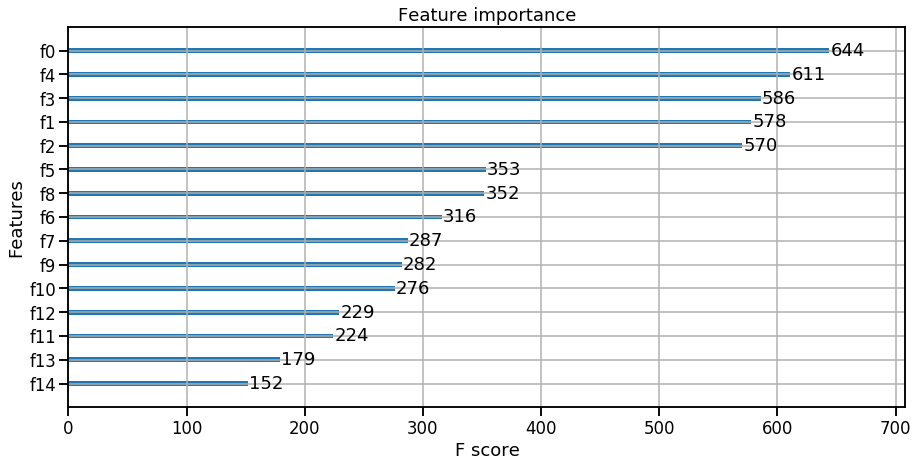
\includegraphics[width=0.8\textwidth]{xgboost_feature_imp}
		\caption{Relative importance for each feature provided by the trained XGBoost model.}
		\label{fig:xgboost_feature_imp}
	\end{adjustwidth}
\end{figure} 

\subsubsection{Obtain one solution from PMAO-5DW}
In pursuit of a single high-quality solution, we proceed even further. We employ the following two schemes to obtain a single high-quality solution by summarizing the five solutions generated by PMAO-5DW.
\begin{enumerate}
\item GRED: Summarize the five candidate trees using greedy consensus method of PAUP* (Phylogenetic Analysis Using PAUP)\footnote{https://paup.phylosolutions.com/}.
	\item AST: Summarize the five candidate trees based on quartet consistency using ASTRAL~\cite{zhang2018astral}, one of the most accurate and widely used coalescent-based methods to infer species trees.
\end{enumerate}
We compare the FN rates of the aforementioned summarizing schemes with PASTA on all BAliBASE 3.0 datasets, except set A to eliminate any bias due to their involvement in training the regression model, in Supplementary Table~\ref{tab:obtain-single-ml} in Appendix~\ref{apendix:pmao}. Then we apply the Friedman Aligned Ranks test followed by Holm's post-hoc procedure on these data and report the results in Table~\ref{tab:test-summary}. We observe that GRED and AST schemes exhibit significantly better performance than PASTA, with GRED being the top performer. However, these schemes are not always able to obtain the best FN rates of PMAO-5DW, and thus we see that PASTA performs better than GRED and AST (Supplementary Table~\ref{tab:obtain-single-ml} in Appendix~\ref{apendix:pmao}) in 37 cases out of 191. This suggests that, although promising, further refinement of this approach or application of other strategies may be in order.

\begin{table}[htbp]
 \centering
  \small
  \caption{\underline{Friedman Aligned Ranks test (Column 2):} Friedman Aligned ranks (lower is better) of PASTA and two schemes for summarizing five solutions generated by PMAO-5DW based on FN rates reported in Supplementary Table~\ref{tab:obtain-single-ml} in Appendix~\ref{apendix:pmao}. We also show the computed statistics and corresponding $ p $-value.
	\underline{Holm's post-hoc procedure (Columns 3 - 5):} Comparison among PASTA and two summarizing schemes using the Holm's post-hoc procedures. Each entry shows the adjusted $p$-value which indicates the significance of the difference in performance between two methods.}
    \begin{tabular}{|l|r|ccc|}
    \hline
    \multicolumn{1}{|c|}{1} & \multicolumn{1}{c|}{2} & \multicolumn{1}{c|}{3} & \multicolumn{1}{c|}{4} & 5 \\
    \hline
	\multirow{2}{*}{\makecell{Methods}} & \multirow{2}{*}{\makecell{Friedman\\Aligned rank*}} & \multicolumn{3}{c|}{Holm's adjusted $p$-value} \\
\cline{3-5}          &       & \multicolumn{1}{l|}{GRED} & \multicolumn{1}{l|}{AST} & \multicolumn{1}{l|}{PASTA} \\
    \hline
    GRED  & 263.9922 & \multicolumn{1}{c|}{-} & \multicolumn{1}{r|}{0.5982} & \multicolumn{1}{r|}{\cellcolor[rgb]{ 0,  .69,  .314}0.0012} \\
    \hline
    AST   & 272.9189 & \multicolumn{1}{r|}{0.5982} & \multicolumn{1}{c|}{-} & \multicolumn{1}{r|}{\cellcolor[rgb]{ 0,  .69,  .314}0.0051} \\
    \hline
    PASTA & 324.0890 & \multicolumn{1}{r|}{\cellcolor[rgb]{ 0,  .69,  .314}0.0012} & \multicolumn{1}{r|}{\cellcolor[rgb]{ 0,  .69,  .314}0.0051} & - \\
    \hline
    *Statistic & 10.7149 & \multicolumn{3}{c|}{\multirow{2}{*}{N/A}} \\
\cline{1-2}    *$p$-value & 0.0047 & \multicolumn{3}{c|}{} \\
    \hline
    \end{tabular}\label{tab:test-summary}
\end{table} 

\section{Conclusion}
In this chapter, we focused on inferring better phylogenetic trees from MSAs by incorporating many application-aware objective functions through decomposition-based MO principles. In this direction, we developed the PMAO framework, which is based on PASTA, one of the most celebrated algorithms/tools in this regard. We evaluated the PMAO framework and examined its capability to yield high-quality tress by experimenting on the widely used BAliBASE 3.0 benchmark. The PMAO framework, like other MO algorithms, outputs a good number of alternative solutions that are equivalent (usually referred to as the non-dominated solutions) in the context of the conflicting objectives considered in the MO framework. Some of these solutions may however be of relatively lower quality from the application perspective. To this end, we innovatively employ machine learning to help PMAO generate only five solutions encompassing at least one top-quality solution. Furthermore, summarizing those five solutions to obtain a single one can offer better accuracy over PASTA in most of the cases, although not as good as the overall PMAO best. In the next chapter, we will develop a flexible software framework for inferring better phylogenetic trees from unaligned sequences by hybridizing any iterative MSA method with MO optimization strategy and leveraging multiple Maximum Likelihood hypotheses.
% In the future, we endeavor to enhance the summarizing approach and apply other strategies of leveraging the alternative MSAs/trees to single out the overall PMAO best solution.Notably, in this work we primarily focused on improving the accuracy of PASTA and hence designed our experiments accordingly. We did not experiment scalability as PASTA is considered as a highly scalable tool.

%We believe this work will further encourage researchers to investigate various application-aware measures for computing and evaluating MSAs. Such effort will potentially prompt more experimental studies addressing specific application domains and ultimately will propel our understanding of MSAs and their impact in various domains in bioinformatics, i.e., phylogeny estimation, protein structure, and function prediction, orthology prediction, etc. Consequently, we expect to see new scalable MSA tools by simultaneously optimizing multiple appropriate optimization criteria.
 

%\bibliographystyle{plain}
%\bibliography{mybibfile}



